\documentclass[twoside]{book}

% Packages required by doxygen
\usepackage{fixltx2e}
\usepackage{calc}
\usepackage{doxygen}
\usepackage[export]{adjustbox} % also loads graphicx
\usepackage{graphicx}
\usepackage[utf8]{inputenc}
\usepackage{makeidx}
\usepackage{multicol}
\usepackage{multirow}
\PassOptionsToPackage{warn}{textcomp}
\usepackage{textcomp}
\usepackage[nointegrals]{wasysym}
\usepackage[table]{xcolor}

% Font selection
\usepackage[T1]{fontenc}
\usepackage[scaled=.90]{helvet}
\usepackage{courier}
\usepackage{amssymb}
\usepackage{sectsty}
\renewcommand{\familydefault}{\sfdefault}
\allsectionsfont{%
  \fontseries{bc}\selectfont%
  \color{darkgray}%
}
\renewcommand{\DoxyLabelFont}{%
  \fontseries{bc}\selectfont%
  \color{darkgray}%
}
\newcommand{\+}{\discretionary{\mbox{\scriptsize$\hookleftarrow$}}{}{}}

% Page & text layout
\usepackage{geometry}
\geometry{%
  a4paper,%
  top=2.5cm,%
  bottom=2.5cm,%
  left=2.5cm,%
  right=2.5cm%
}
\tolerance=750
\hfuzz=15pt
\hbadness=750
\setlength{\emergencystretch}{15pt}
\setlength{\parindent}{0cm}
\setlength{\parskip}{3ex plus 2ex minus 2ex}
\makeatletter
\renewcommand{\paragraph}{%
  \@startsection{paragraph}{4}{0ex}{-1.0ex}{1.0ex}{%
    \normalfont\normalsize\bfseries\SS@parafont%
  }%
}
\renewcommand{\subparagraph}{%
  \@startsection{subparagraph}{5}{0ex}{-1.0ex}{1.0ex}{%
    \normalfont\normalsize\bfseries\SS@subparafont%
  }%
}
\makeatother

% Headers & footers
\usepackage{fancyhdr}
\pagestyle{fancyplain}
\fancyhead[LE]{\fancyplain{}{\bfseries\thepage}}
\fancyhead[CE]{\fancyplain{}{}}
\fancyhead[RE]{\fancyplain{}{\bfseries\leftmark}}
\fancyhead[LO]{\fancyplain{}{\bfseries\rightmark}}
\fancyhead[CO]{\fancyplain{}{}}
\fancyhead[RO]{\fancyplain{}{\bfseries\thepage}}
\fancyfoot[LE]{\fancyplain{}{}}
\fancyfoot[CE]{\fancyplain{}{}}
\fancyfoot[RE]{\fancyplain{}{\bfseries\scriptsize Generated by Doxygen }}
\fancyfoot[LO]{\fancyplain{}{\bfseries\scriptsize Generated by Doxygen }}
\fancyfoot[CO]{\fancyplain{}{}}
\fancyfoot[RO]{\fancyplain{}{}}
\renewcommand{\footrulewidth}{0.4pt}
\renewcommand{\chaptermark}[1]{%
  \markboth{#1}{}%
}
\renewcommand{\sectionmark}[1]{%
  \markright{\thesection\ #1}%
}

% Indices & bibliography
\usepackage{natbib}
\usepackage[titles]{tocloft}
\setcounter{tocdepth}{3}
\setcounter{secnumdepth}{5}
\makeindex

% Hyperlinks (required, but should be loaded last)
\usepackage{ifpdf}
\ifpdf
  \usepackage[pdftex,pagebackref=true]{hyperref}
\else
  \usepackage[ps2pdf,pagebackref=true]{hyperref}
\fi
\hypersetup{%
  colorlinks=true,%
  linkcolor=blue,%
  citecolor=blue,%
  unicode%
}

% Custom commands
\newcommand{\clearemptydoublepage}{%
  \newpage{\pagestyle{empty}\cleardoublepage}%
}

\usepackage{caption}
\captionsetup{labelsep=space,justification=centering,font={bf},singlelinecheck=off,skip=4pt,position=top}

%===== C O N T E N T S =====

\begin{document}

% Titlepage & ToC
\hypersetup{pageanchor=false,
             bookmarksnumbered=true,
             pdfencoding=unicode
            }
\pagenumbering{alph}
\begin{titlepage}
\vspace*{7cm}
\begin{center}%
{\Large J\+SL }\\
\vspace*{1cm}
{\large Generated by Doxygen 1.8.13}\\
\end{center}
\end{titlepage}
\clearemptydoublepage
\pagenumbering{roman}
\tableofcontents
\clearemptydoublepage
\pagenumbering{arabic}
\hypersetup{pageanchor=true}

%--- Begin generated contents ---
\chapter{Namespace Index}
\doxysection{Namespace List}
Here is a list of all namespaces with brief descriptions\+:\begin{DoxyCompactList}
\item\contentsline{section}{\mbox{\hyperlink{namespaceJSL}{J\+SL}} }{\pageref{namespaceJSL}}{}
\item\contentsline{section}{\mbox{\hyperlink{namespaceJSL__Testing}{J\+S\+L\+\_\+\+Testing}} }{\pageref{namespaceJSL__Testing}}{}
\end{DoxyCompactList}

\chapter{Hierarchical Index}
\doxysection{Class Hierarchy}
This inheritance list is sorted roughly, but not completely, alphabetically\+:\begin{DoxyCompactList}
\item \contentsline{section}{J\+SL\+::Argument\+Interface}{\pageref{classJSL_1_1ArgumentInterface}}{}
\begin{DoxyCompactList}
\item \contentsline{section}{J\+SL\+::Argument$<$ T $>$}{\pageref{classJSL_1_1Argument}}{}
\end{DoxyCompactList}
\item \contentsline{section}{J\+SL\+::mkdir\+Return}{\pageref{structJSL_1_1mkdirReturn}}{}
\item \contentsline{section}{J\+SL\+::Unit\+Test}{\pageref{classJSL_1_1UnitTest}}{}
\begin{DoxyCompactList}
\item \contentsline{section}{J\+S\+L\+\_\+\+Testing\+::I\+O\+Test}{\pageref{classJSL__Testing_1_1IOTest}}{}
\item \contentsline{section}{J\+S\+L\+\_\+\+Testing\+::Meta\+Test}{\pageref{classJSL__Testing_1_1MetaTest}}{}
\item \contentsline{section}{J\+S\+L\+\_\+\+Testing\+::String\+Test}{\pageref{classJSL__Testing_1_1StringTest}}{}
\end{DoxyCompactList}
\end{DoxyCompactList}

\chapter{Data Structure Index}
\section{Data Structures}
Here are the data structures with brief descriptions\+:\begin{DoxyCompactList}
\item\contentsline{section}{\hyperlink{classJSL_1_1Argument}{J\+S\+L\+::\+Argument$<$ T $>$} }{\pageref{classJSL_1_1Argument}}{}
\item\contentsline{section}{\hyperlink{classJSL_1_1ArgumentInterface}{J\+S\+L\+::\+Argument\+Interface} }{\pageref{classJSL_1_1ArgumentInterface}}{}
\item\contentsline{section}{\hyperlink{structJSL_1_1mkdirReturn}{J\+S\+L\+::mkdir\+Return} }{\pageref{structJSL_1_1mkdirReturn}}{}
\end{DoxyCompactList}

\chapter{File Index}
\doxysection{File List}
Here is a list of all files with brief descriptions\+:\begin{DoxyCompactList}
\item\contentsline{section}{/\+Users/jf20/\+Documents/\+JSL/\mbox{\hyperlink{JSL_8h}{JSL.\+h}} }{\pageref{JSL_8h}}{}
\item\contentsline{section}{/\+Users/jf20/\+Documents/\+JSL/\+Array/\mbox{\hyperlink{Array_8h}{Array.\+h}} }{\pageref{Array_8h}}{}
\item\contentsline{section}{/\+Users/jf20/\+Documents/\+JSL/\+Array/\mbox{\hyperlink{VectorSearches_8h}{Vector\+Searches.\+h}} }{\pageref{VectorSearches_8h}}{}
\item\contentsline{section}{/\+Users/jf20/\+Documents/\+JSL/\+Command\+Args/\mbox{\hyperlink{Argument_8h}{Argument.\+h}} }{\pageref{Argument_8h}}{}
\item\contentsline{section}{/\+Users/jf20/\+Documents/\+JSL/\+Command\+Args/\mbox{\hyperlink{CommandArgs_8h}{Command\+Args.\+h}} }{\pageref{CommandArgs_8h}}{}
\item\contentsline{section}{/\+Users/jf20/\+Documents/\+JSL/\+Display/\mbox{\hyperlink{clearScreen_8h}{clear\+Screen.\+h}} }{\pageref{clearScreen_8h}}{}
\item\contentsline{section}{/\+Users/jf20/\+Documents/\+JSL/\+Display/\mbox{\hyperlink{Display_8h}{Display.\+h}} }{\pageref{Display_8h}}{}
\item\contentsline{section}{/\+Users/jf20/\+Documents/\+JSL/\+Display/\mbox{\hyperlink{ProgressBar_8h}{Progress\+Bar.\+h}} }{\pageref{ProgressBar_8h}}{}
\item\contentsline{section}{/\+Users/jf20/\+Documents/\+JSL/\+File\+IO/\mbox{\hyperlink{FileIO_8h}{File\+IO.\+h}} }{\pageref{FileIO_8h}}{}
\item\contentsline{section}{/\+Users/jf20/\+Documents/\+JSL/\+File\+IO/\mbox{\hyperlink{fileWriter_8h}{file\+Writer.\+h}} }{\pageref{fileWriter_8h}}{}
\item\contentsline{section}{/\+Users/jf20/\+Documents/\+JSL/\+File\+IO/\mbox{\hyperlink{LineReader_8h}{Line\+Reader.\+h}} }{\pageref{LineReader_8h}}{}
\item\contentsline{section}{/\+Users/jf20/\+Documents/\+JSL/\+File\+IO/\mbox{\hyperlink{locationExists_8h}{location\+Exists.\+h}} }{\pageref{locationExists_8h}}{}
\item\contentsline{section}{/\+Users/jf20/\+Documents/\+JSL/\+File\+IO/\mbox{\hyperlink{mkdir_8h}{mkdir.\+h}} }{\pageref{mkdir_8h}}{}
\item\contentsline{section}{/\+Users/jf20/\+Documents/\+JSL/gnuplot/\mbox{\hyperlink{axis_8h}{axis.\+h}} }{\pageref{axis_8h}}{}
\item\contentsline{section}{/\+Users/jf20/\+Documents/\+JSL/gnuplot/\mbox{\hyperlink{gnuplot_8h}{gnuplot.\+h}} }{\pageref{gnuplot_8h}}{}
\item\contentsline{section}{/\+Users/jf20/\+Documents/\+JSL/gnuplot/\mbox{\hyperlink{gnuplotMain_8h}{gnuplot\+Main.\+h}} }{\pageref{gnuplotMain_8h}}{}
\item\contentsline{section}{/\+Users/jf20/\+Documents/\+JSL/gnuplot/\mbox{\hyperlink{PlotData_8h}{Plot\+Data.\+h}} }{\pageref{PlotData_8h}}{}
\item\contentsline{section}{/\+Users/jf20/\+Documents/\+JSL/\+Maths/\mbox{\hyperlink{Maths_8h}{Maths.\+h}} }{\pageref{Maths_8h}}{}
\item\contentsline{section}{/\+Users/jf20/\+Documents/\+JSL/\+Maths/\mbox{\hyperlink{matrix_8h}{matrix.\+h}} }{\pageref{matrix_8h}}{}
\item\contentsline{section}{/\+Users/jf20/\+Documents/\+JSL/\+Maths/\mbox{\hyperlink{MiscFunctions_8h}{Misc\+Functions.\+h}} }{\pageref{MiscFunctions_8h}}{}
\item\contentsline{section}{/\+Users/jf20/\+Documents/\+JSL/\+Maths/\mbox{\hyperlink{Q__temp_8h}{Q\+\_\+temp.\+h}} }{\pageref{Q__temp_8h}}{}
\item\contentsline{section}{/\+Users/jf20/\+Documents/\+JSL/\+Maths/\mbox{\hyperlink{vector_8h}{vector.\+h}} }{\pageref{vector_8h}}{}
\item\contentsline{section}{/\+Users/jf20/\+Documents/\+JSL/\+Strings/\mbox{\hyperlink{split_8h}{split.\+h}} }{\pageref{split_8h}}{}
\item\contentsline{section}{/\+Users/jf20/\+Documents/\+JSL/\+Strings/\mbox{\hyperlink{Strings_8h}{Strings.\+h}} }{\pageref{Strings_8h}}{}
\item\contentsline{section}{/\+Users/jf20/\+Documents/\+JSL/\+Strings/\mbox{\hyperlink{Time_8h}{Time.\+h}} }{\pageref{Time_8h}}{}
\item\contentsline{section}{/\+Users/jf20/\+Documents/\+JSL/\+System/\mbox{\hyperlink{assert_8h}{assert.\+h}} }{\pageref{assert_8h}}{}
\item\contentsline{section}{/\+Users/jf20/\+Documents/\+JSL/\+System/\mbox{\hyperlink{error_8h}{error.\+h}} }{\pageref{error_8h}}{}
\item\contentsline{section}{/\+Users/jf20/\+Documents/\+JSL/\+System/\mbox{\hyperlink{rm_8h}{rm.\+h}} }{\pageref{rm_8h}}{}
\item\contentsline{section}{/\+Users/jf20/\+Documents/\+JSL/\+System/\mbox{\hyperlink{System_8h}{System.\+h}} }{\pageref{System_8h}}{}
\item\contentsline{section}{/\+Users/jf20/\+Documents/\+JSL/\+System/\mbox{\hyperlink{systemCall_8h}{system\+Call.\+h}} }{\pageref{systemCall_8h}}{}
\item\contentsline{section}{/\+Users/jf20/\+Documents/\+JSL/\+Testing/\mbox{\hyperlink{Testing_8h}{Testing.\+h}} }{\pageref{Testing_8h}}{}
\item\contentsline{section}{/\+Users/jf20/\+Documents/\+JSL/\+Testing/\mbox{\hyperlink{Testing__UnitTests_8h}{Testing\+\_\+\+Unit\+Tests.\+h}} }{\pageref{Testing__UnitTests_8h}}{}
\item\contentsline{section}{/\+Users/jf20/\+Documents/\+JSL/\+Testing/\mbox{\hyperlink{UnitTest_8h}{Unit\+Test.\+h}} }{\pageref{UnitTest_8h}}{}
\end{DoxyCompactList}

\chapter{Namespace Documentation}
\hypertarget{namespaceJSL}{}\doxysection{JSL Namespace Reference}
\label{namespaceJSL}\index{JSL@{JSL}}
\doxysubsection*{Namespaces}
\begin{DoxyCompactItemize}
\item 
namespace \mbox{\hyperlink{namespaceJSL_1_1Fonts}{Fonts}}
\item 
namespace \mbox{\hyperlink{namespaceJSL_1_1internal}{internal}}
\item 
namespace \mbox{\hyperlink{namespaceJSL_1_1LineProperties}{Line\+Properties}}
\end{DoxyCompactItemize}
\doxysubsection*{Data Structures}
\begin{DoxyCompactItemize}
\item 
class \mbox{\hyperlink{classJSL_1_1Argument}{Argument}}
\item 
class \mbox{\hyperlink{classJSL_1_1ArgumentInterface}{Argument\+Interface}}
\item 
class \mbox{\hyperlink{classJSL_1_1Axis}{Axis}}
\item 
class \mbox{\hyperlink{classJSL_1_1gnuplot}{gnuplot}}
\item 
class \mbox{\hyperlink{classJSL_1_1Matrix}{Matrix}}
\item 
struct \mbox{\hyperlink{structJSL_1_1mkdirReturn}{mkdir\+Return}}
\begin{DoxyCompactList}\small\item\em A wrapper for the return type of mkdir\+Safely() \end{DoxyCompactList}\item 
struct \mbox{\hyperlink{structJSL_1_1NameValuePair}{Name\+Value\+Pair}}
\item 
class \mbox{\hyperlink{classJSL_1_1PlotData}{Plot\+Data}}
\item 
class \mbox{\hyperlink{classJSL_1_1ProgressBar}{Progress\+Bar}}
\item 
class \mbox{\hyperlink{classJSL_1_1Quaternion}{Quaternion}}
\item 
class \mbox{\hyperlink{classJSL_1_1UnitTest}{Unit\+Test}}
\item 
class \mbox{\hyperlink{classJSL_1_1Vector}{Vector}}
\end{DoxyCompactItemize}
\doxysubsection*{Enumerations}
\begin{DoxyCompactItemize}
\item 
enum \mbox{\hyperlink{namespaceJSL_a871354b683a8bee0151dbfbbde49beda}{Plot\+Type}} \{ \mbox{\hyperlink{namespaceJSL_a871354b683a8bee0151dbfbbde49bedaafa1098e16302d619cc16c6117128c7e2}{Line}}
, \mbox{\hyperlink{namespaceJSL_a871354b683a8bee0151dbfbbde49bedaa523747d04b06019ae6db545703793d22}{Scatter\+Point}}
 \}
\item 
enum \mbox{\hyperlink{namespaceJSL_ad5aeae8cb562d6f38c724cbdc51d81f8}{Property}} \{ \mbox{\hyperlink{namespaceJSL_ad5aeae8cb562d6f38c724cbdc51d81f8ae7660181e67b34cc8012e44899358c0a}{Colour}}
, \mbox{\hyperlink{namespaceJSL_ad5aeae8cb562d6f38c724cbdc51d81f8a22d189b48d50314bdd20b34e9a40e4a5}{Pen\+Size}}
, \mbox{\hyperlink{namespaceJSL_ad5aeae8cb562d6f38c724cbdc51d81f8ab516e098813c27967b8e649b94f98db8}{Pen\+Type}}
, \mbox{\hyperlink{namespaceJSL_ad5aeae8cb562d6f38c724cbdc51d81f8afadeba2e8b035dc3c761f416c88a293d}{Legend}}
 \}
\item 
enum \mbox{\hyperlink{namespaceJSL_acbabfae0b320d418d49485b7c50bc355}{Line\+Type}} \{ \newline
\mbox{\hyperlink{namespaceJSL_acbabfae0b320d418d49485b7c50bc355aaf6d64d28f76aa54961a419d3d9e17b5}{Solid}}
, \mbox{\hyperlink{namespaceJSL_acbabfae0b320d418d49485b7c50bc355a5d77703e9d097677886b897d9a2eeb62}{Dash}}
, \mbox{\hyperlink{namespaceJSL_acbabfae0b320d418d49485b7c50bc355af0b887cb0d75c330317bc843146bfc92}{Dash\+Dot}}
, \mbox{\hyperlink{namespaceJSL_acbabfae0b320d418d49485b7c50bc355ac3cd9b153ce73b7d8dd0485ae186379d}{Dotted}}
, \newline
\mbox{\hyperlink{namespaceJSL_acbabfae0b320d418d49485b7c50bc355a48afd9609abb3d990c826b2c74850d3e}{Dash\+Dot\+Dot}}
 \}
\item 
enum \mbox{\hyperlink{namespaceJSL_a086efb36ddb107d45961a6b46932c526}{Scatter\+Type}} \{ \newline
\mbox{\hyperlink{namespaceJSL_a086efb36ddb107d45961a6b46932c526a7d6491e51b0151fad51114bdc9fe0006}{Dot}}
, \mbox{\hyperlink{namespaceJSL_a086efb36ddb107d45961a6b46932c526ac54fadde63eae4fbfb5090af9e2c8c68}{Plus}}
, \mbox{\hyperlink{namespaceJSL_a086efb36ddb107d45961a6b46932c526af2349f50039f930d90a39a689282aaf8}{Cross}}
, \mbox{\hyperlink{namespaceJSL_a086efb36ddb107d45961a6b46932c526a3d4283b7785e19142f43a8d705f45128}{Star}}
, \newline
\mbox{\hyperlink{namespaceJSL_a086efb36ddb107d45961a6b46932c526af5af415948dea41c775febe11df59707}{Open\+Square}}
, \mbox{\hyperlink{namespaceJSL_a086efb36ddb107d45961a6b46932c526ab2977a42bdf7f8cafd62d56eb573d71a}{Filled\+Square}}
, \mbox{\hyperlink{namespaceJSL_a086efb36ddb107d45961a6b46932c526a24102e043f642c5aadf0a5184838e065}{Open\+Circle}}
, \mbox{\hyperlink{namespaceJSL_a086efb36ddb107d45961a6b46932c526a1e5a2218783d5197e73aab6b16f3add3}{Filled\+Circle}}
, \newline
\mbox{\hyperlink{namespaceJSL_a086efb36ddb107d45961a6b46932c526a163fb60ab5d5beca95d7afa4c97d6fda}{Open\+Delta}}
, \mbox{\hyperlink{namespaceJSL_a086efb36ddb107d45961a6b46932c526abc2204e7d338e5c0f3c5b524c3250352}{Filled\+Delta}}
, \mbox{\hyperlink{namespaceJSL_a086efb36ddb107d45961a6b46932c526ae6f313a61f49260feabbe0252daebf39}{Open\+Nabla}}
, \mbox{\hyperlink{namespaceJSL_a086efb36ddb107d45961a6b46932c526ac57738c0de5dcd2b52aedd0ac353fcd8}{Filled\+Nabla}}
, \newline
\mbox{\hyperlink{namespaceJSL_a086efb36ddb107d45961a6b46932c526aede7da49ec9867bc58a9883ac6f7fd12}{Open\+Diamond}}
, \mbox{\hyperlink{namespaceJSL_a086efb36ddb107d45961a6b46932c526a9ba302e97b23281952e4e194387808b2}{Filled\+Diamond}}
 \}
\item 
enum \mbox{\hyperlink{namespaceJSL_a5059dbafa288b9b3beac1746f4acae61}{Error\+Code}} \{ \newline
\mbox{\hyperlink{namespaceJSL_a5059dbafa288b9b3beac1746f4acae61a0a229ef32833c9a64ed38080ba87b196}{JSLError}}
, \mbox{\hyperlink{namespaceJSL_a5059dbafa288b9b3beac1746f4acae61ab2e398994d8ffbb8c17109c9ec85ed30}{System\+Error}}
, \mbox{\hyperlink{namespaceJSL_a5059dbafa288b9b3beac1746f4acae61afec2ceb4545826a8594a9dc7a7b1c702}{Overrun\+Error}}
, \mbox{\hyperlink{namespaceJSL_a5059dbafa288b9b3beac1746f4acae61a007fec64442c721c18380cb70c51a443}{Failed\+Assertion}}
, \newline
\mbox{\hyperlink{namespaceJSL_a5059dbafa288b9b3beac1746f4acae61a7da39e712d8960d161fbef3305d793a4}{IOError}}
 \}
\end{DoxyCompactItemize}
\doxysubsection*{Functions}
\begin{DoxyCompactItemize}
\item 
{\footnotesize template$<$class T $>$ }\\int \mbox{\hyperlink{namespaceJSL_a428e6ac7fa22e5c5aa3bceb9e17fe970}{Find\+XInY}} (T x, const std\+::vector$<$ T $>$ \&y)
\item 
{\footnotesize template$<$typename T $>$ }\\std\+::vector$<$ size\+\_\+t $>$ \mbox{\hyperlink{namespaceJSL_a1d104ebd2bbb9ec6eade1abbb59fa84e}{Sort\+Indices}} (const std\+::vector$<$ T $>$ \&v)
\item 
int \mbox{\hyperlink{namespaceJSL_a6e3dd386e7ab4be6fae6e0bdf8c98e91}{Upper\+Bound\+Locator}} (double val, const std\+::vector$<$ double $>$ \&val\+Array)
\begin{DoxyCompactList}\small\item\em Similar to Find\+XInY except where you do not expect an exact match. Searches through an (assumed sorted) vector and locates the first value greater than or equal to the target value, else returns the index of the final value in the array. \end{DoxyCompactList}\item 
void \mbox{\hyperlink{namespaceJSL_a405f53748ca024b70694b0534cfcf4a3}{jump\+Line\+Up}} ()
\item 
void \mbox{\hyperlink{namespaceJSL_a071b279ad5267ce66ff86c614952a3ed}{clear\+Screen}} ()
\item 
void \mbox{\hyperlink{namespaceJSL_ae38780f94d60045b904b289eb3ab8eda}{delete\+Line}} ()
\item 
void \mbox{\hyperlink{namespaceJSL_a47d8cb112d513ee5a3ae38ca6a89743d}{initialise\+File}} (const std\+::string \&filename)
\item 
void \mbox{\hyperlink{namespaceJSL_a838b3a913896993bc008408d164ec19d}{write\+String\+To\+File}} (const std\+::string \&filename, const std\+::string \&content)
\item 
{\footnotesize template$<$class T $>$ }\\void \mbox{\hyperlink{namespaceJSL_a1d611217d83275af846cbc091ff98f53}{write\+Vector\+To\+File}} (const std\+::string \&filename, const std\+::vector$<$ T $>$ \&content\+Vector, const std\+::string \&delimiter, bool include\+Terminal\+Line\+Break)
\item 
{\footnotesize template$<$typename T , typename... Ts$>$ }\\void \mbox{\hyperlink{namespaceJSL_a425710dc6536490f1c1d6a5ce621f0e3}{write\+Multi\+Vector\+To\+File}} (const std\+::string \&filename, const std\+::string \&delimiter, const std\+::vector$<$ T $>$ \&v1, const std\+::vector$<$ Ts $>$ \&... vecs)
\item 
{\footnotesize template$<$class T $>$ }\\void \mbox{\hyperlink{namespaceJSL_ae790600d9f16e338cfc8b50cd1bfc8f4}{write\+Matrix\+To\+File}} (const std\+::string \&filename, const std\+::vector$<$ std\+::vector$<$ T $>$ $>$ content\+Matrix, const std\+::string \&column\+Delimiter, const std\+::string \&row\+Delimiter)
\item 
bool \mbox{\hyperlink{namespaceJSL_a1752cd7c6e1134da51e9307527e0d788}{location\+Exists}} (const std\+::string \&filename)
\item 
\mbox{\hyperlink{structJSL_1_1mkdirReturn}{mkdir\+Return}} \mbox{\hyperlink{namespaceJSL_abf525d02b8c49f21ef7faa68b7571f93}{mkdir}} (std\+::string directory)
\item 
bool \mbox{\hyperlink{namespaceJSL_a682c8bb3fff54370f38dcb16794fc7c5}{operator==}} (const \mbox{\hyperlink{classJSL_1_1Matrix}{Matrix}} \&lhs, const \mbox{\hyperlink{classJSL_1_1Matrix}{Matrix}} \&rhs)
\item 
bool \mbox{\hyperlink{namespaceJSL_a8b19814a4b6cb667d1e27133acc38513}{operator!=}} (const \mbox{\hyperlink{classJSL_1_1Matrix}{Matrix}} \&lhs, const \mbox{\hyperlink{classJSL_1_1Matrix}{Matrix}} \&rhs)
\item 
bool \mbox{\hyperlink{namespaceJSL_a38d1bbf23dc57ec028ea8d91a9688957}{Matrix\+Sizes\+Equal}} (const \mbox{\hyperlink{classJSL_1_1Matrix}{Matrix}} \&m1, const \mbox{\hyperlink{classJSL_1_1Matrix}{Matrix}} \&m2)
\item 
\mbox{\hyperlink{classJSL_1_1Matrix}{Matrix}} \mbox{\hyperlink{namespaceJSL_ad1bcc74167579ecff71209bf8c9c47a3}{operator+}} (const \mbox{\hyperlink{classJSL_1_1Matrix}{Matrix}} \&lhs, const \mbox{\hyperlink{classJSL_1_1Matrix}{Matrix}} \&rhs)
\begin{DoxyCompactList}\small\item\em Performs obvious matrix addition (a+b)\+\_\+ij = a\+\_\+ij + b\+\_\+ij. Throws an error if the matrices are not the same size. \end{DoxyCompactList}\item 
\mbox{\hyperlink{classJSL_1_1Matrix}{Matrix}} \mbox{\hyperlink{namespaceJSL_a4f1a2a224c7f6a8c57627b03594cd89f}{operator-\/}} (const \mbox{\hyperlink{classJSL_1_1Matrix}{Matrix}} \&lhs, const \mbox{\hyperlink{classJSL_1_1Matrix}{Matrix}} \&rhs)
\begin{DoxyCompactList}\small\item\em Performs obvious matrix subtraction (a-\/b)\+\_\+ij = a\+\_\+ij -\/ b\+\_\+ij. Throws an error if the matrices are not the same size. \end{DoxyCompactList}\item 
\mbox{\hyperlink{classJSL_1_1Matrix}{Matrix}} \mbox{\hyperlink{namespaceJSL_ad779a68a2d565490f76dd16adfc3091e}{operator+}} (const \mbox{\hyperlink{classJSL_1_1Matrix}{Matrix}} \&lhs, const double \&scalar)
\begin{DoxyCompactList}\small\item\em Adds the value of scalar to every element in the matrix. \end{DoxyCompactList}\item 
\mbox{\hyperlink{classJSL_1_1Matrix}{Matrix}} \mbox{\hyperlink{namespaceJSL_a95d670e99aed43f857d8ba5e6f3d7897}{operator$\ast$}} (const \mbox{\hyperlink{classJSL_1_1Matrix}{Matrix}} \&lhs, const \mbox{\hyperlink{classJSL_1_1Matrix}{Matrix}} \&rhs)
\item 
\mbox{\hyperlink{classJSL_1_1Vector}{Vector}} \mbox{\hyperlink{namespaceJSL_a823f5e48d384320644698917c0a1c85c}{operator$\ast$}} (const \mbox{\hyperlink{classJSL_1_1Matrix}{Matrix}} \&lhs, const \mbox{\hyperlink{classJSL_1_1Vector}{Vector}} \&rhs)
\item 
\mbox{\hyperlink{classJSL_1_1Matrix}{Matrix}} \mbox{\hyperlink{namespaceJSL_a5f6c1988cf84b088617e0f12fc1e98da}{operator+}} (const double \&scalar, const \mbox{\hyperlink{classJSL_1_1Matrix}{Matrix}} \&rhs)
\begin{DoxyCompactList}\small\item\em Exactly equivalent to \mbox{\hyperlink{namespaceJSL_ad779a68a2d565490f76dd16adfc3091e}{JSL\+::operator+(const Matrix \&lhs, const double \&scalar)}}, just swapped around. \end{DoxyCompactList}\item 
\mbox{\hyperlink{classJSL_1_1Matrix}{Matrix}} \mbox{\hyperlink{namespaceJSL_a6d5304adbdadcb062246266f4ece24a1}{operator-\/}} (const \mbox{\hyperlink{classJSL_1_1Matrix}{Matrix}} \&lhs, const double \&scalar)
\begin{DoxyCompactList}\small\item\em Subtracts the value of scalar to every element in the \mbox{\hyperlink{classJSL_1_1Matrix}{Matrix}}. \end{DoxyCompactList}\item 
\mbox{\hyperlink{classJSL_1_1Matrix}{Matrix}} \mbox{\hyperlink{namespaceJSL_a80fcd230a03dd81f1c37fec030619bf9}{operator$\ast$}} (const double \&scalar, const \mbox{\hyperlink{classJSL_1_1Matrix}{Matrix}} \&rhs)
\begin{DoxyCompactList}\small\item\em Naive element-\/wise scalar multiplication. \end{DoxyCompactList}\item 
\mbox{\hyperlink{classJSL_1_1Matrix}{Matrix}} \mbox{\hyperlink{namespaceJSL_a69548e09ba5835ee87ac4d28907b5435}{operator$\ast$}} (const \mbox{\hyperlink{classJSL_1_1Matrix}{Matrix}} \&lhs, const double \&scalar)
\begin{DoxyCompactList}\small\item\em Alias of \mbox{\hyperlink{namespaceJSL_a5f6c1988cf84b088617e0f12fc1e98da}{JSL\+::operator+(const double \&scalar,const Matrix \&rhs)}} with the operation order swapped around. \end{DoxyCompactList}\item 
\mbox{\hyperlink{classJSL_1_1Matrix}{Matrix}} \mbox{\hyperlink{namespaceJSL_ab1f3153179f59c59a0c2a5e553889eb1}{operator/}} (const \mbox{\hyperlink{classJSL_1_1Matrix}{Matrix}} \&lhs, const double \&scalar)
\begin{DoxyCompactList}\small\item\em Essentially an alias for \mbox{\hyperlink{namespaceJSL_a5f6c1988cf84b088617e0f12fc1e98da}{JSL\+::operator+(const double \&scalar,const Matrix \&rhs)}} with the scalar set to one-\/over itself, i.\+e. pointwise division of the provided matrix. \end{DoxyCompactList}\item 
\mbox{\hyperlink{classJSL_1_1Matrix}{Matrix}} \mbox{\hyperlink{namespaceJSL_aebaffa5dc8073b816908a9708a36b7bf}{operator-\/}} (const double \&scalar, const \mbox{\hyperlink{classJSL_1_1Matrix}{Matrix}} \&rhs)
\begin{DoxyCompactList}\small\item\em A slightly odd operation (included for completeness) -\/ adds the value of scalar to the negative of the elements of the vector. \end{DoxyCompactList}\item 
std\+::ostream \& \mbox{\hyperlink{namespaceJSL_a7e357c34e91d1eb03c15ca437a285ea1}{operator$<$$<$}} (std\+::ostream \&os, const \mbox{\hyperlink{classJSL_1_1Matrix}{Matrix}} \&obj)
\begin{DoxyCompactList}\small\item\em Calls \mbox{\hyperlink{classJSL_1_1Matrix_abcf44559767ab6939851f0d3b60c6fa8}{JSL\+::\+Matrix\+::to\+\_\+string()}} and then passes it to the provided stream, enabling sweet, smooth output such as std\+::cout \texorpdfstring{$<$}{<}\texorpdfstring{$<$}{<} M \texorpdfstring{$<$}{<}\texorpdfstring{$<$}{<} std\+::endl. \end{DoxyCompactList}\item 
double \mbox{\hyperlink{namespaceJSL_a017f24cfdf73ecc218aab718c1badd89}{Fraction\+Bounder}} (double a)
\item 
\mbox{\hyperlink{classJSL_1_1Quaternion}{Quaternion}} \mbox{\hyperlink{namespaceJSL_aff956bc38fdc0a19f41e202699560dff}{operator$\ast$}} (const \mbox{\hyperlink{classJSL_1_1Quaternion}{Quaternion}} \&lhs, const \mbox{\hyperlink{classJSL_1_1Quaternion}{Quaternion}} \&rhs)
\item 
\mbox{\hyperlink{classJSL_1_1Quaternion}{Quaternion}} \mbox{\hyperlink{namespaceJSL_a87842870ba7998a0ec521782b2d2f621}{operator$\ast$}} (const \mbox{\hyperlink{classJSL_1_1Matrix}{JSL\+::\+Matrix}} \&lhs, const \mbox{\hyperlink{classJSL_1_1Quaternion}{Quaternion}} \&rhs)
\item 
\mbox{\hyperlink{classJSL_1_1Quaternion}{Quaternion}} \mbox{\hyperlink{namespaceJSL_a68fed2d9fae3ec9612dd8e8282cf1336}{operator/}} (const \mbox{\hyperlink{classJSL_1_1Quaternion}{Quaternion}} \&lhs, const \mbox{\hyperlink{classJSL_1_1Quaternion}{Quaternion}} \&rhs)
\item 
\mbox{\hyperlink{classJSL_1_1Quaternion}{Quaternion}} \mbox{\hyperlink{namespaceJSL_a943a21cab5e9abe4331b20d37cd3f8a1}{exp}} (const \mbox{\hyperlink{classJSL_1_1Quaternion}{JSL\+::\+Quaternion}} \&a)
\item 
double \mbox{\hyperlink{namespaceJSL_aeae64b7e0cfdc1ab5f35cca90c32d9f6}{Vector\+Dot\+Product}} (const \mbox{\hyperlink{classJSL_1_1Vector}{Vector}} \&lhs, const \mbox{\hyperlink{classJSL_1_1Vector}{Vector}} \&rhs)
\begin{DoxyCompactList}\small\item\em The standard dot product on R$^\wedge$n. \end{DoxyCompactList}\item 
\mbox{\hyperlink{classJSL_1_1Vector}{Vector}} \mbox{\hyperlink{namespaceJSL_aa7816eb0cd81b74241ce460237990e70}{Vector\+Cross\+Product}} (const \mbox{\hyperlink{classJSL_1_1Vector}{Vector}} \&lhs, const \mbox{\hyperlink{classJSL_1_1Vector}{Vector}} \&rhs)
\begin{DoxyCompactList}\small\item\em The standard cross product -- only defined on R$^\wedge$3 (throws an error else) \end{DoxyCompactList}\item 
double \mbox{\hyperlink{namespaceJSL_a09355c91f84fd99d4634bf9189fef51d}{Angle\+Between\+Vectors}} (const \mbox{\hyperlink{classJSL_1_1Vector}{Vector}} \&lhs, const \mbox{\hyperlink{classJSL_1_1Vector}{Vector}} \&rhs)
\begin{DoxyCompactList}\small\item\em Uses \mbox{\hyperlink{classJSL_1_1Vector_aa8af717591f5548ff471b6e4b28d7f9c}{Vector\+::\+Norm()}} and \mbox{\hyperlink{namespaceJSL_aeae64b7e0cfdc1ab5f35cca90c32d9f6}{Vector\+Dot\+Product()}} to extract an angle between the vectors. \end{DoxyCompactList}\item 
bool \mbox{\hyperlink{namespaceJSL_a7fad54be308ccb76f68933d91c3c542f}{operator==}} (const \mbox{\hyperlink{classJSL_1_1Vector}{Vector}} \&lhs, const \mbox{\hyperlink{classJSL_1_1Vector}{Vector}} \&rhs)
\item 
bool \mbox{\hyperlink{namespaceJSL_a394a4f9cee0747c76d1190b0365c7b5a}{operator!=}} (const \mbox{\hyperlink{classJSL_1_1Vector}{Vector}} \&lhs, const \mbox{\hyperlink{classJSL_1_1Vector}{Vector}} \&rhs)
\item 
\mbox{\hyperlink{classJSL_1_1Vector}{Vector}} \mbox{\hyperlink{namespaceJSL_ae6530b77174d0dfae8e0d6e2a810f672}{operator+}} (const \mbox{\hyperlink{classJSL_1_1Vector}{Vector}} \&lhs, const \mbox{\hyperlink{classJSL_1_1Vector}{Vector}} \&rhs)
\begin{DoxyCompactList}\small\item\em Performs obvious vector addition (a+b)\+\_\+i = a\+\_\+i + b\+\_\+i. Throws an error if the vectors are not the same size. \end{DoxyCompactList}\item 
\mbox{\hyperlink{classJSL_1_1Vector}{Vector}} \mbox{\hyperlink{namespaceJSL_a1d8393f2865dc23e7975ad041e341ba5}{operator-\/}} (const \mbox{\hyperlink{classJSL_1_1Vector}{Vector}} \&lhs, const \mbox{\hyperlink{classJSL_1_1Vector}{Vector}} \&rhs)
\begin{DoxyCompactList}\small\item\em Performs obvious vector subtraction (a-\/b)\+\_\+i = a\+\_\+i -\/ b\+\_\+i. Throws an error if the vectors are not the same size. \end{DoxyCompactList}\item 
\mbox{\hyperlink{classJSL_1_1Vector}{Vector}} \mbox{\hyperlink{namespaceJSL_a4b293e2ac3df51113e80022cb3c2ac99}{operator+}} (const \mbox{\hyperlink{classJSL_1_1Vector}{Vector}} \&lhs, const double \&scalar)
\begin{DoxyCompactList}\small\item\em Adds the value of scalar to every element in the vector. \end{DoxyCompactList}\item 
\mbox{\hyperlink{classJSL_1_1Vector}{Vector}} \mbox{\hyperlink{namespaceJSL_ac5ceabb8b9e657c5e2d0faf9b20a36e8}{operator+}} (const double \&scalar, const \mbox{\hyperlink{classJSL_1_1Vector}{Vector}} \&rhs)
\begin{DoxyCompactList}\small\item\em Exactly equivalent to \mbox{\hyperlink{namespaceJSL_a4b293e2ac3df51113e80022cb3c2ac99}{JSL\+::operator+(const Vector \&lhs, const double \&scalar)}}, just swapped around. \end{DoxyCompactList}\item 
\mbox{\hyperlink{classJSL_1_1Vector}{Vector}} \mbox{\hyperlink{namespaceJSL_ac6bd9311dd73aa6227d826bdb94e748d}{operator-\/}} (const \mbox{\hyperlink{classJSL_1_1Vector}{Vector}} \&lhs, const double \&scalar)
\begin{DoxyCompactList}\small\item\em Subtracts the value of scalar to every element in the vector. \end{DoxyCompactList}\item 
\mbox{\hyperlink{classJSL_1_1Vector}{Vector}} \mbox{\hyperlink{namespaceJSL_ab3d17c5cc03a2048e8637d2054fbc138}{operator-\/}} (const double \&scalar, const \mbox{\hyperlink{classJSL_1_1Vector}{Vector}} \&rhs)
\begin{DoxyCompactList}\small\item\em A slightly odd operation (included for completeness) -\/ adds the value of scalar to the negative of the elements of the vector. \end{DoxyCompactList}\item 
\mbox{\hyperlink{classJSL_1_1Vector}{Vector}} \mbox{\hyperlink{namespaceJSL_ab4eefbed468f275164855895335b8a29}{operator$\ast$}} (const double \&scalar, const \mbox{\hyperlink{classJSL_1_1Vector}{Vector}} \&rhs)
\begin{DoxyCompactList}\small\item\em Naive element-\/wise scalar multiplication. \end{DoxyCompactList}\item 
\mbox{\hyperlink{classJSL_1_1Vector}{Vector}} \mbox{\hyperlink{namespaceJSL_afc5e092de4a9bdc5795d40ee0f51c7b9}{operator$\ast$}} (const \mbox{\hyperlink{classJSL_1_1Vector}{Vector}} \&lhs, const double \&scalar)
\begin{DoxyCompactList}\small\item\em Alias of \mbox{\hyperlink{namespaceJSL_ac5ceabb8b9e657c5e2d0faf9b20a36e8}{JSL\+::operator+(const double \&scalar,const Vector \&rhs)}} with the operation order swapped around. \end{DoxyCompactList}\item 
\mbox{\hyperlink{classJSL_1_1Vector}{Vector}} \mbox{\hyperlink{namespaceJSL_a1427fd44260592b7d65d27946969fba1}{operator/}} (const \mbox{\hyperlink{classJSL_1_1Vector}{Vector}} \&lhs, const double \&scalar)
\begin{DoxyCompactList}\small\item\em Essentially an alias for \mbox{\hyperlink{namespaceJSL_ac5ceabb8b9e657c5e2d0faf9b20a36e8}{JSL\+::operator+(const double \&scalar,const Vector \&rhs)}} with the scalar set to one-\/over itself, i.\+e. pointwise division of the provided vector. \end{DoxyCompactList}\item 
\mbox{\hyperlink{classJSL_1_1Vector}{Vector}} \mbox{\hyperlink{namespaceJSL_a6fd4487b0a8ac5713df4a37079287913}{Hadamard}} (const \mbox{\hyperlink{classJSL_1_1Vector}{Vector}} \&lhs, const \mbox{\hyperlink{classJSL_1_1Vector}{Vector}} \&rhs)
\begin{DoxyCompactList}\small\item\em Executes the pointwise (Hadamard) product of two vectors. \end{DoxyCompactList}\item 
std\+::ostream \& \mbox{\hyperlink{namespaceJSL_ad01cc2984ad2ce5a85fb31960835dd04}{operator$<$$<$}} (std\+::ostream \&os, const \mbox{\hyperlink{classJSL_1_1Vector}{Vector}} \&obj)
\begin{DoxyCompactList}\small\item\em Calls \mbox{\hyperlink{classJSL_1_1Vector_a73579b4a194cc924341806a5d9ea3817}{JSL\+::\+Vector\+::to\+\_\+string()}} and then passes it to the provided stream, enabling sweet, smooth output such as std\+::cout \texorpdfstring{$<$}{<}\texorpdfstring{$<$}{<} v1 \texorpdfstring{$<$}{<}\texorpdfstring{$<$}{<} std\+::endl. \end{DoxyCompactList}\item 
\mbox{\hyperlink{classJSL_1_1Vector}{Vector}} \mbox{\hyperlink{namespaceJSL_a941b0093a8d1298a0dc0c4403f63a826}{Element\+Wise\+Operation}} (\mbox{\hyperlink{classJSL_1_1Vector}{Vector}} input, double($\ast$function)(double))
\begin{DoxyCompactList}\small\item\em A nice way to perform a simple function on every element of a vector. \end{DoxyCompactList}\item 
std\+::vector$<$ std\+::string $>$ \mbox{\hyperlink{namespaceJSL_aa37a5ffd99a34e2f12377c9f00b31c50}{split}} (const std\+::string \&s, char delimiter)
\item 
std\+::string \mbox{\hyperlink{namespaceJSL_ae58b7096986a16b70a27e1609eff3014}{Current\+Time}} ()
\item 
std\+::string \mbox{\hyperlink{namespaceJSL_ad7ff2220bbab0294b95b9aa85332a222}{Format\+Duration}} (int time\+In\+Seconds)
\item 
std\+::string \mbox{\hyperlink{namespaceJSL_ae7af96a0311784e019209221335f76d9}{Format\+Clock}} (std\+::chrono\+::time\+\_\+point$<$ std\+::chrono\+::system\+\_\+clock $>$ start, std\+::chrono\+::time\+\_\+point$<$ std\+::chrono\+::system\+\_\+clock $>$ end)
\item 
{\footnotesize template$<$typename... Ts$>$ }\\void \mbox{\hyperlink{namespaceJSL_a1a7afe30fd764dc4151982a2631f08d3}{Assert}} (std\+::string assertion\+Message, Ts... args)
\item 
void \mbox{\hyperlink{namespaceJSL_a5783bc90550deca94c1790e581fb707d}{Error}} (\mbox{\hyperlink{namespaceJSL_a5059dbafa288b9b3beac1746f4acae61}{Error\+Code}} code, const std\+::string \&message)
\item 
void \mbox{\hyperlink{namespaceJSL_a0241a3cc1fa4dd4d319ab8686d1cfaa3}{Error}} (const std\+::string \&message)
\item 
void \mbox{\hyperlink{namespaceJSL_ae48b92e64fb9d321121df976b770efa6}{rm}} (std\+::string location, bool recursive)
\item 
void \mbox{\hyperlink{namespaceJSL_a5cd4ed117decf1140104ad8566b589ac}{system\+Call}} (const std\+::string \&command)
\end{DoxyCompactItemize}
\doxysubsection*{Variables}
\begin{DoxyCompactItemize}
\item 
const std\+::vector$<$ std\+::string $>$ \mbox{\hyperlink{namespaceJSL_a606f5a286ccd4cf3d860d2efde2eac82}{Error\+Names}} = \{\char`\"{}ERROR\char`\"{}, \char`\"{}SYSTEM ERROR\char`\"{}, \char`\"{}OVERRUN ERROR\char`\"{}, \char`\"{}FAILED ASSERTION\char`\"{},\char`\"{}\mbox{\hyperlink{namespaceJSL_a5059dbafa288b9b3beac1746f4acae61a7da39e712d8960d161fbef3305d793a4}{IOError}}\char`\"{}\}
\end{DoxyCompactItemize}


\doxysubsection{Enumeration Type Documentation}
\mbox{\Hypertarget{namespaceJSL_a5059dbafa288b9b3beac1746f4acae61}\label{namespaceJSL_a5059dbafa288b9b3beac1746f4acae61}} 
\index{JSL@{JSL}!ErrorCode@{ErrorCode}}
\index{ErrorCode@{ErrorCode}!JSL@{JSL}}
\doxysubsubsection{\texorpdfstring{ErrorCode}{ErrorCode}}
{\footnotesize\ttfamily enum \mbox{\hyperlink{namespaceJSL_a5059dbafa288b9b3beac1746f4acae61}{JSL\+::\+Error\+Code}}}

\begin{DoxyEnumFields}{Enumerator}
\raisebox{\heightof{T}}[0pt][0pt]{\index{JSLError@{JSLError}!JSL@{JSL}}\index{JSL@{JSL}!JSLError@{JSLError}}}\mbox{\Hypertarget{namespaceJSL_a5059dbafa288b9b3beac1746f4acae61a0a229ef32833c9a64ed38080ba87b196}\label{namespaceJSL_a5059dbafa288b9b3beac1746f4acae61a0a229ef32833c9a64ed38080ba87b196}} 
JSLError&\\
\hline

\raisebox{\heightof{T}}[0pt][0pt]{\index{SystemError@{SystemError}!JSL@{JSL}}\index{JSL@{JSL}!SystemError@{SystemError}}}\mbox{\Hypertarget{namespaceJSL_a5059dbafa288b9b3beac1746f4acae61ab2e398994d8ffbb8c17109c9ec85ed30}\label{namespaceJSL_a5059dbafa288b9b3beac1746f4acae61ab2e398994d8ffbb8c17109c9ec85ed30}} 
System\+Error&\\
\hline

\raisebox{\heightof{T}}[0pt][0pt]{\index{OverrunError@{OverrunError}!JSL@{JSL}}\index{JSL@{JSL}!OverrunError@{OverrunError}}}\mbox{\Hypertarget{namespaceJSL_a5059dbafa288b9b3beac1746f4acae61afec2ceb4545826a8594a9dc7a7b1c702}\label{namespaceJSL_a5059dbafa288b9b3beac1746f4acae61afec2ceb4545826a8594a9dc7a7b1c702}} 
Overrun\+Error&\\
\hline

\raisebox{\heightof{T}}[0pt][0pt]{\index{FailedAssertion@{FailedAssertion}!JSL@{JSL}}\index{JSL@{JSL}!FailedAssertion@{FailedAssertion}}}\mbox{\Hypertarget{namespaceJSL_a5059dbafa288b9b3beac1746f4acae61a007fec64442c721c18380cb70c51a443}\label{namespaceJSL_a5059dbafa288b9b3beac1746f4acae61a007fec64442c721c18380cb70c51a443}} 
Failed\+Assertion&\\
\hline

\raisebox{\heightof{T}}[0pt][0pt]{\index{IOError@{IOError}!JSL@{JSL}}\index{JSL@{JSL}!IOError@{IOError}}}\mbox{\Hypertarget{namespaceJSL_a5059dbafa288b9b3beac1746f4acae61a7da39e712d8960d161fbef3305d793a4}\label{namespaceJSL_a5059dbafa288b9b3beac1746f4acae61a7da39e712d8960d161fbef3305d793a4}} 
IOError&\\
\hline

\end{DoxyEnumFields}
\mbox{\Hypertarget{namespaceJSL_acbabfae0b320d418d49485b7c50bc355}\label{namespaceJSL_acbabfae0b320d418d49485b7c50bc355}} 
\index{JSL@{JSL}!LineType@{LineType}}
\index{LineType@{LineType}!JSL@{JSL}}
\doxysubsubsection{\texorpdfstring{LineType}{LineType}}
{\footnotesize\ttfamily enum \mbox{\hyperlink{namespaceJSL_acbabfae0b320d418d49485b7c50bc355}{JSL\+::\+Line\+Type}}}

\begin{DoxyEnumFields}{Enumerator}
\raisebox{\heightof{T}}[0pt][0pt]{\index{Solid@{Solid}!JSL@{JSL}}\index{JSL@{JSL}!Solid@{Solid}}}\mbox{\Hypertarget{namespaceJSL_acbabfae0b320d418d49485b7c50bc355aaf6d64d28f76aa54961a419d3d9e17b5}\label{namespaceJSL_acbabfae0b320d418d49485b7c50bc355aaf6d64d28f76aa54961a419d3d9e17b5}} 
Solid&\\
\hline

\raisebox{\heightof{T}}[0pt][0pt]{\index{Dash@{Dash}!JSL@{JSL}}\index{JSL@{JSL}!Dash@{Dash}}}\mbox{\Hypertarget{namespaceJSL_acbabfae0b320d418d49485b7c50bc355a5d77703e9d097677886b897d9a2eeb62}\label{namespaceJSL_acbabfae0b320d418d49485b7c50bc355a5d77703e9d097677886b897d9a2eeb62}} 
Dash&\\
\hline

\raisebox{\heightof{T}}[0pt][0pt]{\index{DashDot@{DashDot}!JSL@{JSL}}\index{JSL@{JSL}!DashDot@{DashDot}}}\mbox{\Hypertarget{namespaceJSL_acbabfae0b320d418d49485b7c50bc355af0b887cb0d75c330317bc843146bfc92}\label{namespaceJSL_acbabfae0b320d418d49485b7c50bc355af0b887cb0d75c330317bc843146bfc92}} 
Dash\+Dot&\\
\hline

\raisebox{\heightof{T}}[0pt][0pt]{\index{Dotted@{Dotted}!JSL@{JSL}}\index{JSL@{JSL}!Dotted@{Dotted}}}\mbox{\Hypertarget{namespaceJSL_acbabfae0b320d418d49485b7c50bc355ac3cd9b153ce73b7d8dd0485ae186379d}\label{namespaceJSL_acbabfae0b320d418d49485b7c50bc355ac3cd9b153ce73b7d8dd0485ae186379d}} 
Dotted&\\
\hline

\raisebox{\heightof{T}}[0pt][0pt]{\index{DashDotDot@{DashDotDot}!JSL@{JSL}}\index{JSL@{JSL}!DashDotDot@{DashDotDot}}}\mbox{\Hypertarget{namespaceJSL_acbabfae0b320d418d49485b7c50bc355a48afd9609abb3d990c826b2c74850d3e}\label{namespaceJSL_acbabfae0b320d418d49485b7c50bc355a48afd9609abb3d990c826b2c74850d3e}} 
Dash\+Dot\+Dot&\\
\hline

\end{DoxyEnumFields}
\mbox{\Hypertarget{namespaceJSL_a871354b683a8bee0151dbfbbde49beda}\label{namespaceJSL_a871354b683a8bee0151dbfbbde49beda}} 
\index{JSL@{JSL}!PlotType@{PlotType}}
\index{PlotType@{PlotType}!JSL@{JSL}}
\doxysubsubsection{\texorpdfstring{PlotType}{PlotType}}
{\footnotesize\ttfamily enum \mbox{\hyperlink{namespaceJSL_a871354b683a8bee0151dbfbbde49beda}{JSL\+::\+Plot\+Type}}}

\begin{DoxyEnumFields}{Enumerator}
\raisebox{\heightof{T}}[0pt][0pt]{\index{Line@{Line}!JSL@{JSL}}\index{JSL@{JSL}!Line@{Line}}}\mbox{\Hypertarget{namespaceJSL_a871354b683a8bee0151dbfbbde49bedaafa1098e16302d619cc16c6117128c7e2}\label{namespaceJSL_a871354b683a8bee0151dbfbbde49bedaafa1098e16302d619cc16c6117128c7e2}} 
Line&\\
\hline

\raisebox{\heightof{T}}[0pt][0pt]{\index{ScatterPoint@{ScatterPoint}!JSL@{JSL}}\index{JSL@{JSL}!ScatterPoint@{ScatterPoint}}}\mbox{\Hypertarget{namespaceJSL_a871354b683a8bee0151dbfbbde49bedaa523747d04b06019ae6db545703793d22}\label{namespaceJSL_a871354b683a8bee0151dbfbbde49bedaa523747d04b06019ae6db545703793d22}} 
Scatter\+Point&\\
\hline

\end{DoxyEnumFields}
\mbox{\Hypertarget{namespaceJSL_ad5aeae8cb562d6f38c724cbdc51d81f8}\label{namespaceJSL_ad5aeae8cb562d6f38c724cbdc51d81f8}} 
\index{JSL@{JSL}!Property@{Property}}
\index{Property@{Property}!JSL@{JSL}}
\doxysubsubsection{\texorpdfstring{Property}{Property}}
{\footnotesize\ttfamily enum \mbox{\hyperlink{namespaceJSL_ad5aeae8cb562d6f38c724cbdc51d81f8}{JSL\+::\+Property}}}

\begin{DoxyEnumFields}{Enumerator}
\raisebox{\heightof{T}}[0pt][0pt]{\index{Colour@{Colour}!JSL@{JSL}}\index{JSL@{JSL}!Colour@{Colour}}}\mbox{\Hypertarget{namespaceJSL_ad5aeae8cb562d6f38c724cbdc51d81f8ae7660181e67b34cc8012e44899358c0a}\label{namespaceJSL_ad5aeae8cb562d6f38c724cbdc51d81f8ae7660181e67b34cc8012e44899358c0a}} 
Colour&\\
\hline

\raisebox{\heightof{T}}[0pt][0pt]{\index{PenSize@{PenSize}!JSL@{JSL}}\index{JSL@{JSL}!PenSize@{PenSize}}}\mbox{\Hypertarget{namespaceJSL_ad5aeae8cb562d6f38c724cbdc51d81f8a22d189b48d50314bdd20b34e9a40e4a5}\label{namespaceJSL_ad5aeae8cb562d6f38c724cbdc51d81f8a22d189b48d50314bdd20b34e9a40e4a5}} 
Pen\+Size&\\
\hline

\raisebox{\heightof{T}}[0pt][0pt]{\index{PenType@{PenType}!JSL@{JSL}}\index{JSL@{JSL}!PenType@{PenType}}}\mbox{\Hypertarget{namespaceJSL_ad5aeae8cb562d6f38c724cbdc51d81f8ab516e098813c27967b8e649b94f98db8}\label{namespaceJSL_ad5aeae8cb562d6f38c724cbdc51d81f8ab516e098813c27967b8e649b94f98db8}} 
Pen\+Type&\\
\hline

\raisebox{\heightof{T}}[0pt][0pt]{\index{Legend@{Legend}!JSL@{JSL}}\index{JSL@{JSL}!Legend@{Legend}}}\mbox{\Hypertarget{namespaceJSL_ad5aeae8cb562d6f38c724cbdc51d81f8afadeba2e8b035dc3c761f416c88a293d}\label{namespaceJSL_ad5aeae8cb562d6f38c724cbdc51d81f8afadeba2e8b035dc3c761f416c88a293d}} 
Legend&\\
\hline

\end{DoxyEnumFields}
\mbox{\Hypertarget{namespaceJSL_a086efb36ddb107d45961a6b46932c526}\label{namespaceJSL_a086efb36ddb107d45961a6b46932c526}} 
\index{JSL@{JSL}!ScatterType@{ScatterType}}
\index{ScatterType@{ScatterType}!JSL@{JSL}}
\doxysubsubsection{\texorpdfstring{ScatterType}{ScatterType}}
{\footnotesize\ttfamily enum \mbox{\hyperlink{namespaceJSL_a086efb36ddb107d45961a6b46932c526}{JSL\+::\+Scatter\+Type}}}

\begin{DoxyEnumFields}{Enumerator}
\raisebox{\heightof{T}}[0pt][0pt]{\index{Dot@{Dot}!JSL@{JSL}}\index{JSL@{JSL}!Dot@{Dot}}}\mbox{\Hypertarget{namespaceJSL_a086efb36ddb107d45961a6b46932c526a7d6491e51b0151fad51114bdc9fe0006}\label{namespaceJSL_a086efb36ddb107d45961a6b46932c526a7d6491e51b0151fad51114bdc9fe0006}} 
Dot&\\
\hline

\raisebox{\heightof{T}}[0pt][0pt]{\index{Plus@{Plus}!JSL@{JSL}}\index{JSL@{JSL}!Plus@{Plus}}}\mbox{\Hypertarget{namespaceJSL_a086efb36ddb107d45961a6b46932c526ac54fadde63eae4fbfb5090af9e2c8c68}\label{namespaceJSL_a086efb36ddb107d45961a6b46932c526ac54fadde63eae4fbfb5090af9e2c8c68}} 
Plus&\\
\hline

\raisebox{\heightof{T}}[0pt][0pt]{\index{Cross@{Cross}!JSL@{JSL}}\index{JSL@{JSL}!Cross@{Cross}}}\mbox{\Hypertarget{namespaceJSL_a086efb36ddb107d45961a6b46932c526af2349f50039f930d90a39a689282aaf8}\label{namespaceJSL_a086efb36ddb107d45961a6b46932c526af2349f50039f930d90a39a689282aaf8}} 
Cross&\\
\hline

\raisebox{\heightof{T}}[0pt][0pt]{\index{Star@{Star}!JSL@{JSL}}\index{JSL@{JSL}!Star@{Star}}}\mbox{\Hypertarget{namespaceJSL_a086efb36ddb107d45961a6b46932c526a3d4283b7785e19142f43a8d705f45128}\label{namespaceJSL_a086efb36ddb107d45961a6b46932c526a3d4283b7785e19142f43a8d705f45128}} 
Star&\\
\hline

\raisebox{\heightof{T}}[0pt][0pt]{\index{OpenSquare@{OpenSquare}!JSL@{JSL}}\index{JSL@{JSL}!OpenSquare@{OpenSquare}}}\mbox{\Hypertarget{namespaceJSL_a086efb36ddb107d45961a6b46932c526af5af415948dea41c775febe11df59707}\label{namespaceJSL_a086efb36ddb107d45961a6b46932c526af5af415948dea41c775febe11df59707}} 
Open\+Square&\\
\hline

\raisebox{\heightof{T}}[0pt][0pt]{\index{FilledSquare@{FilledSquare}!JSL@{JSL}}\index{JSL@{JSL}!FilledSquare@{FilledSquare}}}\mbox{\Hypertarget{namespaceJSL_a086efb36ddb107d45961a6b46932c526ab2977a42bdf7f8cafd62d56eb573d71a}\label{namespaceJSL_a086efb36ddb107d45961a6b46932c526ab2977a42bdf7f8cafd62d56eb573d71a}} 
Filled\+Square&\\
\hline

\raisebox{\heightof{T}}[0pt][0pt]{\index{OpenCircle@{OpenCircle}!JSL@{JSL}}\index{JSL@{JSL}!OpenCircle@{OpenCircle}}}\mbox{\Hypertarget{namespaceJSL_a086efb36ddb107d45961a6b46932c526a24102e043f642c5aadf0a5184838e065}\label{namespaceJSL_a086efb36ddb107d45961a6b46932c526a24102e043f642c5aadf0a5184838e065}} 
Open\+Circle&\\
\hline

\raisebox{\heightof{T}}[0pt][0pt]{\index{FilledCircle@{FilledCircle}!JSL@{JSL}}\index{JSL@{JSL}!FilledCircle@{FilledCircle}}}\mbox{\Hypertarget{namespaceJSL_a086efb36ddb107d45961a6b46932c526a1e5a2218783d5197e73aab6b16f3add3}\label{namespaceJSL_a086efb36ddb107d45961a6b46932c526a1e5a2218783d5197e73aab6b16f3add3}} 
Filled\+Circle&\\
\hline

\raisebox{\heightof{T}}[0pt][0pt]{\index{OpenDelta@{OpenDelta}!JSL@{JSL}}\index{JSL@{JSL}!OpenDelta@{OpenDelta}}}\mbox{\Hypertarget{namespaceJSL_a086efb36ddb107d45961a6b46932c526a163fb60ab5d5beca95d7afa4c97d6fda}\label{namespaceJSL_a086efb36ddb107d45961a6b46932c526a163fb60ab5d5beca95d7afa4c97d6fda}} 
Open\+Delta&\\
\hline

\raisebox{\heightof{T}}[0pt][0pt]{\index{FilledDelta@{FilledDelta}!JSL@{JSL}}\index{JSL@{JSL}!FilledDelta@{FilledDelta}}}\mbox{\Hypertarget{namespaceJSL_a086efb36ddb107d45961a6b46932c526abc2204e7d338e5c0f3c5b524c3250352}\label{namespaceJSL_a086efb36ddb107d45961a6b46932c526abc2204e7d338e5c0f3c5b524c3250352}} 
Filled\+Delta&\\
\hline

\raisebox{\heightof{T}}[0pt][0pt]{\index{OpenNabla@{OpenNabla}!JSL@{JSL}}\index{JSL@{JSL}!OpenNabla@{OpenNabla}}}\mbox{\Hypertarget{namespaceJSL_a086efb36ddb107d45961a6b46932c526ae6f313a61f49260feabbe0252daebf39}\label{namespaceJSL_a086efb36ddb107d45961a6b46932c526ae6f313a61f49260feabbe0252daebf39}} 
Open\+Nabla&\\
\hline

\raisebox{\heightof{T}}[0pt][0pt]{\index{FilledNabla@{FilledNabla}!JSL@{JSL}}\index{JSL@{JSL}!FilledNabla@{FilledNabla}}}\mbox{\Hypertarget{namespaceJSL_a086efb36ddb107d45961a6b46932c526ac57738c0de5dcd2b52aedd0ac353fcd8}\label{namespaceJSL_a086efb36ddb107d45961a6b46932c526ac57738c0de5dcd2b52aedd0ac353fcd8}} 
Filled\+Nabla&\\
\hline

\raisebox{\heightof{T}}[0pt][0pt]{\index{OpenDiamond@{OpenDiamond}!JSL@{JSL}}\index{JSL@{JSL}!OpenDiamond@{OpenDiamond}}}\mbox{\Hypertarget{namespaceJSL_a086efb36ddb107d45961a6b46932c526aede7da49ec9867bc58a9883ac6f7fd12}\label{namespaceJSL_a086efb36ddb107d45961a6b46932c526aede7da49ec9867bc58a9883ac6f7fd12}} 
Open\+Diamond&\\
\hline

\raisebox{\heightof{T}}[0pt][0pt]{\index{FilledDiamond@{FilledDiamond}!JSL@{JSL}}\index{JSL@{JSL}!FilledDiamond@{FilledDiamond}}}\mbox{\Hypertarget{namespaceJSL_a086efb36ddb107d45961a6b46932c526a9ba302e97b23281952e4e194387808b2}\label{namespaceJSL_a086efb36ddb107d45961a6b46932c526a9ba302e97b23281952e4e194387808b2}} 
Filled\+Diamond&\\
\hline

\end{DoxyEnumFields}


\doxysubsection{Function Documentation}
\mbox{\Hypertarget{namespaceJSL_a09355c91f84fd99d4634bf9189fef51d}\label{namespaceJSL_a09355c91f84fd99d4634bf9189fef51d}} 
\index{JSL@{JSL}!AngleBetweenVectors@{AngleBetweenVectors}}
\index{AngleBetweenVectors@{AngleBetweenVectors}!JSL@{JSL}}
\doxysubsubsection{\texorpdfstring{AngleBetweenVectors()}{AngleBetweenVectors()}}
{\footnotesize\ttfamily double JSL\+::\+Angle\+Between\+Vectors (\begin{DoxyParamCaption}\item[{const \mbox{\hyperlink{classJSL_1_1Vector}{Vector}} \&}]{lhs,  }\item[{const \mbox{\hyperlink{classJSL_1_1Vector}{Vector}} \&}]{rhs }\end{DoxyParamCaption})\hspace{0.3cm}{\ttfamily [inline]}}



Uses \mbox{\hyperlink{classJSL_1_1Vector_aa8af717591f5548ff471b6e4b28d7f9c}{Vector\+::\+Norm()}} and \mbox{\hyperlink{namespaceJSL_aeae64b7e0cfdc1ab5f35cca90c32d9f6}{Vector\+Dot\+Product()}} to extract an angle between the vectors. 


\begin{DoxyParams}{Parameters}
{\em lhs} & \mbox{\hyperlink{classJSL_1_1Vector}{Vector}} 1,\\
\hline
{\em rhs} & \mbox{\hyperlink{classJSL_1_1Vector}{Vector}} 2 (order irrelevant) \\
\hline
\end{DoxyParams}
\begin{DoxyReturn}{Returns}
The angle between the two vectors (between 0 and M\+\_\+\+PI) 
\end{DoxyReturn}
\mbox{\Hypertarget{namespaceJSL_a1a7afe30fd764dc4151982a2631f08d3}\label{namespaceJSL_a1a7afe30fd764dc4151982a2631f08d3}} 
\index{JSL@{JSL}!Assert@{Assert}}
\index{Assert@{Assert}!JSL@{JSL}}
\doxysubsubsection{\texorpdfstring{Assert()}{Assert()}}
{\footnotesize\ttfamily template$<$typename... Ts$>$ \\
void JSL\+::\+Assert (\begin{DoxyParamCaption}\item[{std\+::string}]{assertion\+Message,  }\item[{Ts...}]{args }\end{DoxyParamCaption})\hspace{0.3cm}{\ttfamily [inline]}}

\mbox{\Hypertarget{namespaceJSL_a071b279ad5267ce66ff86c614952a3ed}\label{namespaceJSL_a071b279ad5267ce66ff86c614952a3ed}} 
\index{JSL@{JSL}!clearScreen@{clearScreen}}
\index{clearScreen@{clearScreen}!JSL@{JSL}}
\doxysubsubsection{\texorpdfstring{clearScreen()}{clearScreen()}}
{\footnotesize\ttfamily void JSL\+::clear\+Screen (\begin{DoxyParamCaption}{ }\end{DoxyParamCaption})\hspace{0.3cm}{\ttfamily [inline]}}

\mbox{\Hypertarget{namespaceJSL_ae58b7096986a16b70a27e1609eff3014}\label{namespaceJSL_ae58b7096986a16b70a27e1609eff3014}} 
\index{JSL@{JSL}!CurrentTime@{CurrentTime}}
\index{CurrentTime@{CurrentTime}!JSL@{JSL}}
\doxysubsubsection{\texorpdfstring{CurrentTime()}{CurrentTime()}}
{\footnotesize\ttfamily std\+::string JSL\+::\+Current\+Time (\begin{DoxyParamCaption}{ }\end{DoxyParamCaption})\hspace{0.3cm}{\ttfamily [inline]}}

Get current system time in a readable format (note\+: was previously called Print\+Current\+Time) \begin{DoxyReturn}{Returns}
A string of the readable format ~\newline
 
\end{DoxyReturn}
\mbox{\Hypertarget{namespaceJSL_ae38780f94d60045b904b289eb3ab8eda}\label{namespaceJSL_ae38780f94d60045b904b289eb3ab8eda}} 
\index{JSL@{JSL}!deleteLine@{deleteLine}}
\index{deleteLine@{deleteLine}!JSL@{JSL}}
\doxysubsubsection{\texorpdfstring{deleteLine()}{deleteLine()}}
{\footnotesize\ttfamily void JSL\+::delete\+Line (\begin{DoxyParamCaption}{ }\end{DoxyParamCaption})\hspace{0.3cm}{\ttfamily [inline]}}

\mbox{\Hypertarget{namespaceJSL_a941b0093a8d1298a0dc0c4403f63a826}\label{namespaceJSL_a941b0093a8d1298a0dc0c4403f63a826}} 
\index{JSL@{JSL}!ElementWiseOperation@{ElementWiseOperation}}
\index{ElementWiseOperation@{ElementWiseOperation}!JSL@{JSL}}
\doxysubsubsection{\texorpdfstring{ElementWiseOperation()}{ElementWiseOperation()}}
{\footnotesize\ttfamily \mbox{\hyperlink{classJSL_1_1Vector}{Vector}} JSL\+::\+Element\+Wise\+Operation (\begin{DoxyParamCaption}\item[{\mbox{\hyperlink{classJSL_1_1Vector}{Vector}}}]{input,  }\item[{double($\ast$)(double)}]{function }\end{DoxyParamCaption})\hspace{0.3cm}{\ttfamily [inline]}}



A nice way to perform a simple function on every element of a vector. 


\begin{DoxyParams}{Parameters}
{\em input} & the vector on which the operation will be performed\\
\hline
{\em function} & A pointer to a funciton which accepts and returns a double. Can also be a lambda function. \\
\hline
\end{DoxyParams}
\begin{DoxyReturn}{Returns}
The vector y such that y\+\_\+i = f(x\+\_\+i) 
\end{DoxyReturn}
\mbox{\Hypertarget{namespaceJSL_a0241a3cc1fa4dd4d319ab8686d1cfaa3}\label{namespaceJSL_a0241a3cc1fa4dd4d319ab8686d1cfaa3}} 
\index{JSL@{JSL}!Error@{Error}}
\index{Error@{Error}!JSL@{JSL}}
\doxysubsubsection{\texorpdfstring{Error()}{Error()}\hspace{0.1cm}{\footnotesize\ttfamily [1/2]}}
{\footnotesize\ttfamily void JSL\+::\+Error (\begin{DoxyParamCaption}\item[{const std\+::string \&}]{message }\end{DoxyParamCaption})\hspace{0.3cm}{\ttfamily [inline]}}

\mbox{\Hypertarget{namespaceJSL_a5783bc90550deca94c1790e581fb707d}\label{namespaceJSL_a5783bc90550deca94c1790e581fb707d}} 
\index{JSL@{JSL}!Error@{Error}}
\index{Error@{Error}!JSL@{JSL}}
\doxysubsubsection{\texorpdfstring{Error()}{Error()}\hspace{0.1cm}{\footnotesize\ttfamily [2/2]}}
{\footnotesize\ttfamily void JSL\+::\+Error (\begin{DoxyParamCaption}\item[{\mbox{\hyperlink{namespaceJSL_a5059dbafa288b9b3beac1746f4acae61}{Error\+Code}}}]{code,  }\item[{const std\+::string \&}]{message }\end{DoxyParamCaption})\hspace{0.3cm}{\ttfamily [inline]}}

Design \mbox{\Hypertarget{namespaceJSL_a943a21cab5e9abe4331b20d37cd3f8a1}\label{namespaceJSL_a943a21cab5e9abe4331b20d37cd3f8a1}} 
\index{JSL@{JSL}!exp@{exp}}
\index{exp@{exp}!JSL@{JSL}}
\doxysubsubsection{\texorpdfstring{exp()}{exp()}}
{\footnotesize\ttfamily \mbox{\hyperlink{classJSL_1_1Quaternion}{Quaternion}} JSL\+::exp (\begin{DoxyParamCaption}\item[{const \mbox{\hyperlink{classJSL_1_1Quaternion}{JSL\+::\+Quaternion}} \&}]{a }\end{DoxyParamCaption})\hspace{0.3cm}{\ttfamily [inline]}}

\mbox{\Hypertarget{namespaceJSL_a428e6ac7fa22e5c5aa3bceb9e17fe970}\label{namespaceJSL_a428e6ac7fa22e5c5aa3bceb9e17fe970}} 
\index{JSL@{JSL}!FindXInY@{FindXInY}}
\index{FindXInY@{FindXInY}!JSL@{JSL}}
\doxysubsubsection{\texorpdfstring{FindXInY()}{FindXInY()}}
{\footnotesize\ttfamily template$<$class T $>$ \\
int JSL\+::\+Find\+XInY (\begin{DoxyParamCaption}\item[{T}]{x,  }\item[{const std\+::vector$<$ T $>$ \&}]{y }\end{DoxyParamCaption})\hspace{0.3cm}{\ttfamily [inline]}}

\mbox{\Hypertarget{namespaceJSL_ae7af96a0311784e019209221335f76d9}\label{namespaceJSL_ae7af96a0311784e019209221335f76d9}} 
\index{JSL@{JSL}!FormatClock@{FormatClock}}
\index{FormatClock@{FormatClock}!JSL@{JSL}}
\doxysubsubsection{\texorpdfstring{FormatClock()}{FormatClock()}}
{\footnotesize\ttfamily std\+::string JSL\+::\+Format\+Clock (\begin{DoxyParamCaption}\item[{std\+::chrono\+::time\+\_\+point$<$ std\+::chrono\+::system\+\_\+clock $>$}]{start,  }\item[{std\+::chrono\+::time\+\_\+point$<$ std\+::chrono\+::system\+\_\+clock $>$}]{end }\end{DoxyParamCaption})\hspace{0.3cm}{\ttfamily [inline]}}

Calls \mbox{\hyperlink{namespaceJSL_ad7ff2220bbab0294b95b9aa85332a222}{Format\+Duration()}} on the duration of the start and endpoints of a {\ttfamily chrono} stopwatch. 
\begin{DoxyParams}{Parameters}
{\em start} & A {\ttfamily chrono} object representing the start of the duration \\
\hline
{\em end} & The corresponding end-\/point {\ttfamily chrono} \\
\hline
\end{DoxyParams}
\mbox{\Hypertarget{namespaceJSL_ad7ff2220bbab0294b95b9aa85332a222}\label{namespaceJSL_ad7ff2220bbab0294b95b9aa85332a222}} 
\index{JSL@{JSL}!FormatDuration@{FormatDuration}}
\index{FormatDuration@{FormatDuration}!JSL@{JSL}}
\doxysubsubsection{\texorpdfstring{FormatDuration()}{FormatDuration()}}
{\footnotesize\ttfamily std\+::string JSL\+::\+Format\+Duration (\begin{DoxyParamCaption}\item[{int}]{time\+In\+Seconds }\end{DoxyParamCaption})\hspace{0.3cm}{\ttfamily [inline]}}

Given a duration in seconds, convert it into standard Day/\+Hour/\+Minute/\+Second formatted string. Times less than 1 second are reported as \char`\"{}less than 1 second\char`\"{} 
\begin{DoxyParams}{Parameters}
{\em time\+In\+Seconds} & The time to be converted \\
\hline
\end{DoxyParams}
\begin{DoxyReturn}{Returns}
A human-\/readable string equal to the input 
\end{DoxyReturn}
\mbox{\Hypertarget{namespaceJSL_a017f24cfdf73ecc218aab718c1badd89}\label{namespaceJSL_a017f24cfdf73ecc218aab718c1badd89}} 
\index{JSL@{JSL}!FractionBounder@{FractionBounder}}
\index{FractionBounder@{FractionBounder}!JSL@{JSL}}
\doxysubsubsection{\texorpdfstring{FractionBounder()}{FractionBounder()}}
{\footnotesize\ttfamily double JSL\+::\+Fraction\+Bounder (\begin{DoxyParamCaption}\item[{double}]{a }\end{DoxyParamCaption})\hspace{0.3cm}{\ttfamily [inline]}}

\mbox{\Hypertarget{namespaceJSL_a6fd4487b0a8ac5713df4a37079287913}\label{namespaceJSL_a6fd4487b0a8ac5713df4a37079287913}} 
\index{JSL@{JSL}!Hadamard@{Hadamard}}
\index{Hadamard@{Hadamard}!JSL@{JSL}}
\doxysubsubsection{\texorpdfstring{Hadamard()}{Hadamard()}}
{\footnotesize\ttfamily \mbox{\hyperlink{classJSL_1_1Vector}{Vector}} JSL\+::\+Hadamard (\begin{DoxyParamCaption}\item[{const \mbox{\hyperlink{classJSL_1_1Vector}{Vector}} \&}]{lhs,  }\item[{const \mbox{\hyperlink{classJSL_1_1Vector}{Vector}} \&}]{rhs }\end{DoxyParamCaption})\hspace{0.3cm}{\ttfamily [inline]}}



Executes the pointwise (Hadamard) product of two vectors. 


\begin{DoxyParams}{Parameters}
{\em lhs} & The first vector to be multiplied\\
\hline
{\em rhs} & The second vector to be multiplied (order is irrelevant) \\
\hline
\end{DoxyParams}
\begin{DoxyReturn}{Returns}
The vector (lhs $\ast$ rhs)\+\_\+i = lhs\+\_\+i $\ast$ rhs\+\_\+i 
\end{DoxyReturn}
\mbox{\Hypertarget{namespaceJSL_a47d8cb112d513ee5a3ae38ca6a89743d}\label{namespaceJSL_a47d8cb112d513ee5a3ae38ca6a89743d}} 
\index{JSL@{JSL}!initialiseFile@{initialiseFile}}
\index{initialiseFile@{initialiseFile}!JSL@{JSL}}
\doxysubsubsection{\texorpdfstring{initialiseFile()}{initialiseFile()}}
{\footnotesize\ttfamily void JSL\+::initialise\+File (\begin{DoxyParamCaption}\item[{const std\+::string \&}]{filename }\end{DoxyParamCaption})\hspace{0.3cm}{\ttfamily [inline]}}

Creates a blank file at the specified location, overwriting any other file at the given location 
\begin{DoxyParams}{Parameters}
{\em filename} & The file which the system will attempt to open \\
\hline
\end{DoxyParams}
\mbox{\Hypertarget{namespaceJSL_a405f53748ca024b70694b0534cfcf4a3}\label{namespaceJSL_a405f53748ca024b70694b0534cfcf4a3}} 
\index{JSL@{JSL}!jumpLineUp@{jumpLineUp}}
\index{jumpLineUp@{jumpLineUp}!JSL@{JSL}}
\doxysubsubsection{\texorpdfstring{jumpLineUp()}{jumpLineUp()}}
{\footnotesize\ttfamily void JSL\+::jump\+Line\+Up (\begin{DoxyParamCaption}{ }\end{DoxyParamCaption})\hspace{0.3cm}{\ttfamily [inline]}}

\mbox{\Hypertarget{namespaceJSL_a1752cd7c6e1134da51e9307527e0d788}\label{namespaceJSL_a1752cd7c6e1134da51e9307527e0d788}} 
\index{JSL@{JSL}!locationExists@{locationExists}}
\index{locationExists@{locationExists}!JSL@{JSL}}
\doxysubsubsection{\texorpdfstring{locationExists()}{locationExists()}}
{\footnotesize\ttfamily bool JSL\+::location\+Exists (\begin{DoxyParamCaption}\item[{const std\+::string \&}]{filename }\end{DoxyParamCaption})\hspace{0.3cm}{\ttfamily [inline]}}

Checks for the existence of the provided file location -- works on both files and directories. 
\begin{DoxyParams}{Parameters}
{\em filename} & the name of the file or directory to be checked \\
\hline
\end{DoxyParams}
\begin{DoxyReturn}{Returns}
true if location exists (and is accessible), false if not 
\end{DoxyReturn}
\mbox{\Hypertarget{namespaceJSL_a38d1bbf23dc57ec028ea8d91a9688957}\label{namespaceJSL_a38d1bbf23dc57ec028ea8d91a9688957}} 
\index{JSL@{JSL}!MatrixSizesEqual@{MatrixSizesEqual}}
\index{MatrixSizesEqual@{MatrixSizesEqual}!JSL@{JSL}}
\doxysubsubsection{\texorpdfstring{MatrixSizesEqual()}{MatrixSizesEqual()}}
{\footnotesize\ttfamily bool JSL\+::\+Matrix\+Sizes\+Equal (\begin{DoxyParamCaption}\item[{const \mbox{\hyperlink{classJSL_1_1Matrix}{Matrix}} \&}]{m1,  }\item[{const \mbox{\hyperlink{classJSL_1_1Matrix}{Matrix}} \&}]{m2 }\end{DoxyParamCaption})\hspace{0.3cm}{\ttfamily [inline]}}

\mbox{\Hypertarget{namespaceJSL_abf525d02b8c49f21ef7faa68b7571f93}\label{namespaceJSL_abf525d02b8c49f21ef7faa68b7571f93}} 
\index{JSL@{JSL}!mkdir@{mkdir}}
\index{mkdir@{mkdir}!JSL@{JSL}}
\doxysubsubsection{\texorpdfstring{mkdir()}{mkdir()}}
{\footnotesize\ttfamily \mbox{\hyperlink{structJSL_1_1mkdirReturn}{mkdir\+Return}} JSL\+::mkdir (\begin{DoxyParamCaption}\item[{std\+::string}]{directory }\end{DoxyParamCaption})\hspace{0.3cm}{\ttfamily [inline]}}

Checks the status of the target directory, if it does not exist, attempts to create it. Works wherever the {\ttfamily mkdir} command is installed. ~\newline
 
\begin{DoxyParams}{Parameters}
{\em directory} & Path (relative or absolute) to the desired directory \\
\hline
\end{DoxyParams}
\begin{DoxyReturn}{Returns}
A \mbox{\hyperlink{structJSL_1_1mkdirReturn}{mkdir\+Return}} object detailing the success + associated messages for the request 
\end{DoxyReturn}
\mbox{\Hypertarget{namespaceJSL_a8b19814a4b6cb667d1e27133acc38513}\label{namespaceJSL_a8b19814a4b6cb667d1e27133acc38513}} 
\index{JSL@{JSL}!operator"!=@{operator"!=}}
\index{operator"!=@{operator"!=}!JSL@{JSL}}
\doxysubsubsection{\texorpdfstring{operator"!=()}{operator!=()}\hspace{0.1cm}{\footnotesize\ttfamily [1/2]}}
{\footnotesize\ttfamily bool JSL\+::operator!= (\begin{DoxyParamCaption}\item[{const \mbox{\hyperlink{classJSL_1_1Matrix}{Matrix}} \&}]{lhs,  }\item[{const \mbox{\hyperlink{classJSL_1_1Matrix}{Matrix}} \&}]{rhs }\end{DoxyParamCaption})\hspace{0.3cm}{\ttfamily [inline]}}

\mbox{\Hypertarget{namespaceJSL_a394a4f9cee0747c76d1190b0365c7b5a}\label{namespaceJSL_a394a4f9cee0747c76d1190b0365c7b5a}} 
\index{JSL@{JSL}!operator"!=@{operator"!=}}
\index{operator"!=@{operator"!=}!JSL@{JSL}}
\doxysubsubsection{\texorpdfstring{operator"!=()}{operator!=()}\hspace{0.1cm}{\footnotesize\ttfamily [2/2]}}
{\footnotesize\ttfamily bool JSL\+::operator!= (\begin{DoxyParamCaption}\item[{const \mbox{\hyperlink{classJSL_1_1Vector}{Vector}} \&}]{lhs,  }\item[{const \mbox{\hyperlink{classJSL_1_1Vector}{Vector}} \&}]{rhs }\end{DoxyParamCaption})\hspace{0.3cm}{\ttfamily [inline]}}

\mbox{\Hypertarget{namespaceJSL_a80fcd230a03dd81f1c37fec030619bf9}\label{namespaceJSL_a80fcd230a03dd81f1c37fec030619bf9}} 
\index{JSL@{JSL}!operator$\ast$@{operator$\ast$}}
\index{operator$\ast$@{operator$\ast$}!JSL@{JSL}}
\doxysubsubsection{\texorpdfstring{operator$\ast$()}{operator*()}\hspace{0.1cm}{\footnotesize\ttfamily [1/8]}}
{\footnotesize\ttfamily \mbox{\hyperlink{classJSL_1_1Matrix}{Matrix}} JSL\+::operator$\ast$ (\begin{DoxyParamCaption}\item[{const double \&}]{scalar,  }\item[{const \mbox{\hyperlink{classJSL_1_1Matrix}{Matrix}} \&}]{rhs }\end{DoxyParamCaption})\hspace{0.3cm}{\ttfamily [inline]}}



Naive element-\/wise scalar multiplication. 


\begin{DoxyParams}{Parameters}
{\em scalar} & The value to multiply elements by\\
\hline
{\em rhs} & The matrix to multiply \\
\hline
\end{DoxyParams}
\begin{DoxyReturn}{Returns}
The pointwise product of the elements of rhs and the scalar 
\end{DoxyReturn}
\mbox{\Hypertarget{namespaceJSL_ab4eefbed468f275164855895335b8a29}\label{namespaceJSL_ab4eefbed468f275164855895335b8a29}} 
\index{JSL@{JSL}!operator$\ast$@{operator$\ast$}}
\index{operator$\ast$@{operator$\ast$}!JSL@{JSL}}
\doxysubsubsection{\texorpdfstring{operator$\ast$()}{operator*()}\hspace{0.1cm}{\footnotesize\ttfamily [2/8]}}
{\footnotesize\ttfamily \mbox{\hyperlink{classJSL_1_1Vector}{Vector}} JSL\+::operator$\ast$ (\begin{DoxyParamCaption}\item[{const double \&}]{scalar,  }\item[{const \mbox{\hyperlink{classJSL_1_1Vector}{Vector}} \&}]{rhs }\end{DoxyParamCaption})\hspace{0.3cm}{\ttfamily [inline]}}



Naive element-\/wise scalar multiplication. 


\begin{DoxyParams}{Parameters}
{\em scalar} & The value to multiply elements by\\
\hline
{\em rhs} & The vector to multiply \\
\hline
\end{DoxyParams}
\begin{DoxyReturn}{Returns}
The pointwise product of the elements of rhs and the scalar 
\end{DoxyReturn}
\mbox{\Hypertarget{namespaceJSL_a87842870ba7998a0ec521782b2d2f621}\label{namespaceJSL_a87842870ba7998a0ec521782b2d2f621}} 
\index{JSL@{JSL}!operator$\ast$@{operator$\ast$}}
\index{operator$\ast$@{operator$\ast$}!JSL@{JSL}}
\doxysubsubsection{\texorpdfstring{operator$\ast$()}{operator*()}\hspace{0.1cm}{\footnotesize\ttfamily [3/8]}}
{\footnotesize\ttfamily \mbox{\hyperlink{classJSL_1_1Quaternion}{Quaternion}} JSL\+::operator$\ast$ (\begin{DoxyParamCaption}\item[{const \mbox{\hyperlink{classJSL_1_1Matrix}{JSL\+::\+Matrix}} \&}]{lhs,  }\item[{const \mbox{\hyperlink{classJSL_1_1Quaternion}{Quaternion}} \&}]{rhs }\end{DoxyParamCaption})\hspace{0.3cm}{\ttfamily [inline]}}

\mbox{\Hypertarget{namespaceJSL_a69548e09ba5835ee87ac4d28907b5435}\label{namespaceJSL_a69548e09ba5835ee87ac4d28907b5435}} 
\index{JSL@{JSL}!operator$\ast$@{operator$\ast$}}
\index{operator$\ast$@{operator$\ast$}!JSL@{JSL}}
\doxysubsubsection{\texorpdfstring{operator$\ast$()}{operator*()}\hspace{0.1cm}{\footnotesize\ttfamily [4/8]}}
{\footnotesize\ttfamily \mbox{\hyperlink{classJSL_1_1Matrix}{Matrix}} JSL\+::operator$\ast$ (\begin{DoxyParamCaption}\item[{const \mbox{\hyperlink{classJSL_1_1Matrix}{Matrix}} \&}]{lhs,  }\item[{const double \&}]{scalar }\end{DoxyParamCaption})\hspace{0.3cm}{\ttfamily [inline]}}



Alias of \mbox{\hyperlink{namespaceJSL_a5f6c1988cf84b088617e0f12fc1e98da}{JSL\+::operator+(const double \&scalar,const Matrix \&rhs)}} with the operation order swapped around. 


\begin{DoxyParams}{Parameters}
{\em lhs} & The matrix to multiply\\
\hline
{\em scalar} & The value to multiply elements by \\
\hline
\end{DoxyParams}
\begin{DoxyReturn}{Returns}
The pointwise product of the elements of lhs and the scalar 
\end{DoxyReturn}
\mbox{\Hypertarget{namespaceJSL_a95d670e99aed43f857d8ba5e6f3d7897}\label{namespaceJSL_a95d670e99aed43f857d8ba5e6f3d7897}} 
\index{JSL@{JSL}!operator$\ast$@{operator$\ast$}}
\index{operator$\ast$@{operator$\ast$}!JSL@{JSL}}
\doxysubsubsection{\texorpdfstring{operator$\ast$()}{operator*()}\hspace{0.1cm}{\footnotesize\ttfamily [5/8]}}
{\footnotesize\ttfamily \mbox{\hyperlink{classJSL_1_1Matrix}{Matrix}} JSL\+::operator$\ast$ (\begin{DoxyParamCaption}\item[{const \mbox{\hyperlink{classJSL_1_1Matrix}{Matrix}} \&}]{lhs,  }\item[{const \mbox{\hyperlink{classJSL_1_1Matrix}{Matrix}} \&}]{rhs }\end{DoxyParamCaption})\hspace{0.3cm}{\ttfamily [inline]}}

\mbox{\Hypertarget{namespaceJSL_a823f5e48d384320644698917c0a1c85c}\label{namespaceJSL_a823f5e48d384320644698917c0a1c85c}} 
\index{JSL@{JSL}!operator$\ast$@{operator$\ast$}}
\index{operator$\ast$@{operator$\ast$}!JSL@{JSL}}
\doxysubsubsection{\texorpdfstring{operator$\ast$()}{operator*()}\hspace{0.1cm}{\footnotesize\ttfamily [6/8]}}
{\footnotesize\ttfamily \mbox{\hyperlink{classJSL_1_1Vector}{Vector}} JSL\+::operator$\ast$ (\begin{DoxyParamCaption}\item[{const \mbox{\hyperlink{classJSL_1_1Matrix}{Matrix}} \&}]{lhs,  }\item[{const \mbox{\hyperlink{classJSL_1_1Vector}{Vector}} \&}]{rhs }\end{DoxyParamCaption})\hspace{0.3cm}{\ttfamily [inline]}}

\mbox{\Hypertarget{namespaceJSL_aff956bc38fdc0a19f41e202699560dff}\label{namespaceJSL_aff956bc38fdc0a19f41e202699560dff}} 
\index{JSL@{JSL}!operator$\ast$@{operator$\ast$}}
\index{operator$\ast$@{operator$\ast$}!JSL@{JSL}}
\doxysubsubsection{\texorpdfstring{operator$\ast$()}{operator*()}\hspace{0.1cm}{\footnotesize\ttfamily [7/8]}}
{\footnotesize\ttfamily \mbox{\hyperlink{classJSL_1_1Quaternion}{Quaternion}} JSL\+::operator$\ast$ (\begin{DoxyParamCaption}\item[{const \mbox{\hyperlink{classJSL_1_1Quaternion}{Quaternion}} \&}]{lhs,  }\item[{const \mbox{\hyperlink{classJSL_1_1Quaternion}{Quaternion}} \&}]{rhs }\end{DoxyParamCaption})\hspace{0.3cm}{\ttfamily [inline]}}

\mbox{\Hypertarget{namespaceJSL_afc5e092de4a9bdc5795d40ee0f51c7b9}\label{namespaceJSL_afc5e092de4a9bdc5795d40ee0f51c7b9}} 
\index{JSL@{JSL}!operator$\ast$@{operator$\ast$}}
\index{operator$\ast$@{operator$\ast$}!JSL@{JSL}}
\doxysubsubsection{\texorpdfstring{operator$\ast$()}{operator*()}\hspace{0.1cm}{\footnotesize\ttfamily [8/8]}}
{\footnotesize\ttfamily \mbox{\hyperlink{classJSL_1_1Vector}{Vector}} JSL\+::operator$\ast$ (\begin{DoxyParamCaption}\item[{const \mbox{\hyperlink{classJSL_1_1Vector}{Vector}} \&}]{lhs,  }\item[{const double \&}]{scalar }\end{DoxyParamCaption})\hspace{0.3cm}{\ttfamily [inline]}}



Alias of \mbox{\hyperlink{namespaceJSL_ac5ceabb8b9e657c5e2d0faf9b20a36e8}{JSL\+::operator+(const double \&scalar,const Vector \&rhs)}} with the operation order swapped around. 


\begin{DoxyParams}{Parameters}
{\em lhs} & The vector to multiply\\
\hline
{\em scalar} & The value to multiply elements by \\
\hline
\end{DoxyParams}
\begin{DoxyReturn}{Returns}
The pointwise product of the elements of lhs and the scalar 
\end{DoxyReturn}
\mbox{\Hypertarget{namespaceJSL_a5f6c1988cf84b088617e0f12fc1e98da}\label{namespaceJSL_a5f6c1988cf84b088617e0f12fc1e98da}} 
\index{JSL@{JSL}!operator+@{operator+}}
\index{operator+@{operator+}!JSL@{JSL}}
\doxysubsubsection{\texorpdfstring{operator+()}{operator+()}\hspace{0.1cm}{\footnotesize\ttfamily [1/6]}}
{\footnotesize\ttfamily \mbox{\hyperlink{classJSL_1_1Matrix}{Matrix}} JSL\+::operator+ (\begin{DoxyParamCaption}\item[{const double \&}]{scalar,  }\item[{const \mbox{\hyperlink{classJSL_1_1Matrix}{Matrix}} \&}]{rhs }\end{DoxyParamCaption})\hspace{0.3cm}{\ttfamily [inline]}}



Exactly equivalent to \mbox{\hyperlink{namespaceJSL_ad779a68a2d565490f76dd16adfc3091e}{JSL\+::operator+(const Matrix \&lhs, const double \&scalar)}}, just swapped around. 


\begin{DoxyParams}{Parameters}
{\em scalar} & The scalar to be added element-\/wise\\
\hline
{\em rhs} & The matrix to be summed \\
\hline
\end{DoxyParams}
\begin{DoxyReturn}{Returns}
The scalar + rhs 
\end{DoxyReturn}
\mbox{\Hypertarget{namespaceJSL_ac5ceabb8b9e657c5e2d0faf9b20a36e8}\label{namespaceJSL_ac5ceabb8b9e657c5e2d0faf9b20a36e8}} 
\index{JSL@{JSL}!operator+@{operator+}}
\index{operator+@{operator+}!JSL@{JSL}}
\doxysubsubsection{\texorpdfstring{operator+()}{operator+()}\hspace{0.1cm}{\footnotesize\ttfamily [2/6]}}
{\footnotesize\ttfamily \mbox{\hyperlink{classJSL_1_1Vector}{Vector}} JSL\+::operator+ (\begin{DoxyParamCaption}\item[{const double \&}]{scalar,  }\item[{const \mbox{\hyperlink{classJSL_1_1Vector}{Vector}} \&}]{rhs }\end{DoxyParamCaption})\hspace{0.3cm}{\ttfamily [inline]}}



Exactly equivalent to \mbox{\hyperlink{namespaceJSL_a4b293e2ac3df51113e80022cb3c2ac99}{JSL\+::operator+(const Vector \&lhs, const double \&scalar)}}, just swapped around. 


\begin{DoxyParams}{Parameters}
{\em scalar} & The scalar to be added element-\/wise\\
\hline
{\em rhs} & The vector to be summed \\
\hline
\end{DoxyParams}
\begin{DoxyReturn}{Returns}
The scalar + rhs 
\end{DoxyReturn}
\mbox{\Hypertarget{namespaceJSL_ad779a68a2d565490f76dd16adfc3091e}\label{namespaceJSL_ad779a68a2d565490f76dd16adfc3091e}} 
\index{JSL@{JSL}!operator+@{operator+}}
\index{operator+@{operator+}!JSL@{JSL}}
\doxysubsubsection{\texorpdfstring{operator+()}{operator+()}\hspace{0.1cm}{\footnotesize\ttfamily [3/6]}}
{\footnotesize\ttfamily \mbox{\hyperlink{classJSL_1_1Matrix}{Matrix}} JSL\+::operator+ (\begin{DoxyParamCaption}\item[{const \mbox{\hyperlink{classJSL_1_1Matrix}{Matrix}} \&}]{lhs,  }\item[{const double \&}]{scalar }\end{DoxyParamCaption})\hspace{0.3cm}{\ttfamily [inline]}}



Adds the value of scalar to every element in the matrix. 


\begin{DoxyParams}{Parameters}
{\em lhs} & The matrix to be summed\\
\hline
{\em scalar} & The scalar to be added element-\/wise \\
\hline
\end{DoxyParams}
\begin{DoxyReturn}{Returns}
The matrix lhs + scalar 
\end{DoxyReturn}
\mbox{\Hypertarget{namespaceJSL_ad1bcc74167579ecff71209bf8c9c47a3}\label{namespaceJSL_ad1bcc74167579ecff71209bf8c9c47a3}} 
\index{JSL@{JSL}!operator+@{operator+}}
\index{operator+@{operator+}!JSL@{JSL}}
\doxysubsubsection{\texorpdfstring{operator+()}{operator+()}\hspace{0.1cm}{\footnotesize\ttfamily [4/6]}}
{\footnotesize\ttfamily \mbox{\hyperlink{classJSL_1_1Matrix}{Matrix}} JSL\+::operator+ (\begin{DoxyParamCaption}\item[{const \mbox{\hyperlink{classJSL_1_1Matrix}{Matrix}} \&}]{lhs,  }\item[{const \mbox{\hyperlink{classJSL_1_1Matrix}{Matrix}} \&}]{rhs }\end{DoxyParamCaption})\hspace{0.3cm}{\ttfamily [inline]}}



Performs obvious matrix addition (a+b)\+\_\+ij = a\+\_\+ij + b\+\_\+ij. Throws an error if the matrices are not the same size. 


\begin{DoxyParams}{Parameters}
{\em lhs} & The first vector to be summed\\
\hline
{\em rhs} & The second vector to be summed (order is irrelevant) \\
\hline
\end{DoxyParams}
\begin{DoxyReturn}{Returns}
The vector lhs + rhs 
\end{DoxyReturn}
\mbox{\Hypertarget{namespaceJSL_a4b293e2ac3df51113e80022cb3c2ac99}\label{namespaceJSL_a4b293e2ac3df51113e80022cb3c2ac99}} 
\index{JSL@{JSL}!operator+@{operator+}}
\index{operator+@{operator+}!JSL@{JSL}}
\doxysubsubsection{\texorpdfstring{operator+()}{operator+()}\hspace{0.1cm}{\footnotesize\ttfamily [5/6]}}
{\footnotesize\ttfamily \mbox{\hyperlink{classJSL_1_1Vector}{Vector}} JSL\+::operator+ (\begin{DoxyParamCaption}\item[{const \mbox{\hyperlink{classJSL_1_1Vector}{Vector}} \&}]{lhs,  }\item[{const double \&}]{scalar }\end{DoxyParamCaption})\hspace{0.3cm}{\ttfamily [inline]}}



Adds the value of scalar to every element in the vector. 


\begin{DoxyParams}{Parameters}
{\em lhs} & The vector to be summed\\
\hline
{\em scalar} & The scalar to be added element-\/wise \\
\hline
\end{DoxyParams}
\begin{DoxyReturn}{Returns}
The vector lhs + scalar 
\end{DoxyReturn}
\mbox{\Hypertarget{namespaceJSL_ae6530b77174d0dfae8e0d6e2a810f672}\label{namespaceJSL_ae6530b77174d0dfae8e0d6e2a810f672}} 
\index{JSL@{JSL}!operator+@{operator+}}
\index{operator+@{operator+}!JSL@{JSL}}
\doxysubsubsection{\texorpdfstring{operator+()}{operator+()}\hspace{0.1cm}{\footnotesize\ttfamily [6/6]}}
{\footnotesize\ttfamily \mbox{\hyperlink{classJSL_1_1Vector}{Vector}} JSL\+::operator+ (\begin{DoxyParamCaption}\item[{const \mbox{\hyperlink{classJSL_1_1Vector}{Vector}} \&}]{lhs,  }\item[{const \mbox{\hyperlink{classJSL_1_1Vector}{Vector}} \&}]{rhs }\end{DoxyParamCaption})\hspace{0.3cm}{\ttfamily [inline]}}



Performs obvious vector addition (a+b)\+\_\+i = a\+\_\+i + b\+\_\+i. Throws an error if the vectors are not the same size. 


\begin{DoxyParams}{Parameters}
{\em lhs} & The first vector to be summed\\
\hline
{\em rhs} & The second vector to be summed (order is irrelevant) \\
\hline
\end{DoxyParams}
\begin{DoxyReturn}{Returns}
The vector lhs + rhs 
\end{DoxyReturn}
\mbox{\Hypertarget{namespaceJSL_aebaffa5dc8073b816908a9708a36b7bf}\label{namespaceJSL_aebaffa5dc8073b816908a9708a36b7bf}} 
\index{JSL@{JSL}!operator-\/@{operator-\/}}
\index{operator-\/@{operator-\/}!JSL@{JSL}}
\doxysubsubsection{\texorpdfstring{operator-\/()}{operator-()}\hspace{0.1cm}{\footnotesize\ttfamily [1/6]}}
{\footnotesize\ttfamily \mbox{\hyperlink{classJSL_1_1Matrix}{Matrix}} JSL\+::operator-\/ (\begin{DoxyParamCaption}\item[{const double \&}]{scalar,  }\item[{const \mbox{\hyperlink{classJSL_1_1Matrix}{Matrix}} \&}]{rhs }\end{DoxyParamCaption})\hspace{0.3cm}{\ttfamily [inline]}}



A slightly odd operation (included for completeness) -\/ adds the value of scalar to the negative of the elements of the vector. 


\begin{DoxyParams}{Parameters}
{\em scalar} & The value which acts as a base\\
\hline
{\em rhs} & The vector which will be subtracted elementwise from the base scalar \\
\hline
\end{DoxyParams}
\begin{DoxyReturn}{Returns}
The vector scalar -\/ rhs 
\end{DoxyReturn}
\mbox{\Hypertarget{namespaceJSL_ab3d17c5cc03a2048e8637d2054fbc138}\label{namespaceJSL_ab3d17c5cc03a2048e8637d2054fbc138}} 
\index{JSL@{JSL}!operator-\/@{operator-\/}}
\index{operator-\/@{operator-\/}!JSL@{JSL}}
\doxysubsubsection{\texorpdfstring{operator-\/()}{operator-()}\hspace{0.1cm}{\footnotesize\ttfamily [2/6]}}
{\footnotesize\ttfamily \mbox{\hyperlink{classJSL_1_1Vector}{Vector}} JSL\+::operator-\/ (\begin{DoxyParamCaption}\item[{const double \&}]{scalar,  }\item[{const \mbox{\hyperlink{classJSL_1_1Vector}{Vector}} \&}]{rhs }\end{DoxyParamCaption})\hspace{0.3cm}{\ttfamily [inline]}}



A slightly odd operation (included for completeness) -\/ adds the value of scalar to the negative of the elements of the vector. 


\begin{DoxyParams}{Parameters}
{\em scalar} & The value which acts as a base\\
\hline
{\em rhs} & The vector which will be subtracted elementwise from the base scalar \\
\hline
\end{DoxyParams}
\begin{DoxyReturn}{Returns}
The vector scalar -\/ rhs 
\end{DoxyReturn}
\mbox{\Hypertarget{namespaceJSL_a6d5304adbdadcb062246266f4ece24a1}\label{namespaceJSL_a6d5304adbdadcb062246266f4ece24a1}} 
\index{JSL@{JSL}!operator-\/@{operator-\/}}
\index{operator-\/@{operator-\/}!JSL@{JSL}}
\doxysubsubsection{\texorpdfstring{operator-\/()}{operator-()}\hspace{0.1cm}{\footnotesize\ttfamily [3/6]}}
{\footnotesize\ttfamily \mbox{\hyperlink{classJSL_1_1Matrix}{Matrix}} JSL\+::operator-\/ (\begin{DoxyParamCaption}\item[{const \mbox{\hyperlink{classJSL_1_1Matrix}{Matrix}} \&}]{lhs,  }\item[{const double \&}]{scalar }\end{DoxyParamCaption})\hspace{0.3cm}{\ttfamily [inline]}}



Subtracts the value of scalar to every element in the \mbox{\hyperlink{classJSL_1_1Matrix}{Matrix}}. 


\begin{DoxyParams}{Parameters}
{\em lhs} & The base matrix\\
\hline
{\em scalar} & The scalar to be subtracted from the base matrix element wise \\
\hline
\end{DoxyParams}
\begin{DoxyReturn}{Returns}
The vector lhs -\/ scalar. 
\end{DoxyReturn}
\mbox{\Hypertarget{namespaceJSL_a4f1a2a224c7f6a8c57627b03594cd89f}\label{namespaceJSL_a4f1a2a224c7f6a8c57627b03594cd89f}} 
\index{JSL@{JSL}!operator-\/@{operator-\/}}
\index{operator-\/@{operator-\/}!JSL@{JSL}}
\doxysubsubsection{\texorpdfstring{operator-\/()}{operator-()}\hspace{0.1cm}{\footnotesize\ttfamily [4/6]}}
{\footnotesize\ttfamily \mbox{\hyperlink{classJSL_1_1Matrix}{Matrix}} JSL\+::operator-\/ (\begin{DoxyParamCaption}\item[{const \mbox{\hyperlink{classJSL_1_1Matrix}{Matrix}} \&}]{lhs,  }\item[{const \mbox{\hyperlink{classJSL_1_1Matrix}{Matrix}} \&}]{rhs }\end{DoxyParamCaption})\hspace{0.3cm}{\ttfamily [inline]}}



Performs obvious matrix subtraction (a-\/b)\+\_\+ij = a\+\_\+ij -\/ b\+\_\+ij. Throws an error if the matrices are not the same size. 


\begin{DoxyParams}{Parameters}
{\em lhs} & The first vector\\
\hline
{\em rhs} & The vector to be subtracted from the first \\
\hline
\end{DoxyParams}
\begin{DoxyReturn}{Returns}
The matrix lhs -\/ rhs 
\end{DoxyReturn}
\mbox{\Hypertarget{namespaceJSL_ac6bd9311dd73aa6227d826bdb94e748d}\label{namespaceJSL_ac6bd9311dd73aa6227d826bdb94e748d}} 
\index{JSL@{JSL}!operator-\/@{operator-\/}}
\index{operator-\/@{operator-\/}!JSL@{JSL}}
\doxysubsubsection{\texorpdfstring{operator-\/()}{operator-()}\hspace{0.1cm}{\footnotesize\ttfamily [5/6]}}
{\footnotesize\ttfamily \mbox{\hyperlink{classJSL_1_1Vector}{Vector}} JSL\+::operator-\/ (\begin{DoxyParamCaption}\item[{const \mbox{\hyperlink{classJSL_1_1Vector}{Vector}} \&}]{lhs,  }\item[{const double \&}]{scalar }\end{DoxyParamCaption})\hspace{0.3cm}{\ttfamily [inline]}}



Subtracts the value of scalar to every element in the vector. 


\begin{DoxyParams}{Parameters}
{\em lhs} & The base vector\\
\hline
{\em scalar} & The scalar to be subtracted from the base vector element wise \\
\hline
\end{DoxyParams}
\begin{DoxyReturn}{Returns}
The vector lhs -\/ scalar. 
\end{DoxyReturn}
\mbox{\Hypertarget{namespaceJSL_a1d8393f2865dc23e7975ad041e341ba5}\label{namespaceJSL_a1d8393f2865dc23e7975ad041e341ba5}} 
\index{JSL@{JSL}!operator-\/@{operator-\/}}
\index{operator-\/@{operator-\/}!JSL@{JSL}}
\doxysubsubsection{\texorpdfstring{operator-\/()}{operator-()}\hspace{0.1cm}{\footnotesize\ttfamily [6/6]}}
{\footnotesize\ttfamily \mbox{\hyperlink{classJSL_1_1Vector}{Vector}} JSL\+::operator-\/ (\begin{DoxyParamCaption}\item[{const \mbox{\hyperlink{classJSL_1_1Vector}{Vector}} \&}]{lhs,  }\item[{const \mbox{\hyperlink{classJSL_1_1Vector}{Vector}} \&}]{rhs }\end{DoxyParamCaption})\hspace{0.3cm}{\ttfamily [inline]}}



Performs obvious vector subtraction (a-\/b)\+\_\+i = a\+\_\+i -\/ b\+\_\+i. Throws an error if the vectors are not the same size. 


\begin{DoxyParams}{Parameters}
{\em lhs} & The base vector\\
\hline
{\em rhs} & The vector to be subtracted from the base vector (order does matter!) \\
\hline
\end{DoxyParams}
\begin{DoxyReturn}{Returns}
The vector lhs -\/ rhs. 
\end{DoxyReturn}
\mbox{\Hypertarget{namespaceJSL_ab1f3153179f59c59a0c2a5e553889eb1}\label{namespaceJSL_ab1f3153179f59c59a0c2a5e553889eb1}} 
\index{JSL@{JSL}!operator/@{operator/}}
\index{operator/@{operator/}!JSL@{JSL}}
\doxysubsubsection{\texorpdfstring{operator/()}{operator/()}\hspace{0.1cm}{\footnotesize\ttfamily [1/3]}}
{\footnotesize\ttfamily \mbox{\hyperlink{classJSL_1_1Matrix}{Matrix}} JSL\+::operator/ (\begin{DoxyParamCaption}\item[{const \mbox{\hyperlink{classJSL_1_1Matrix}{Matrix}} \&}]{lhs,  }\item[{const double \&}]{scalar }\end{DoxyParamCaption})\hspace{0.3cm}{\ttfamily [inline]}}



Essentially an alias for \mbox{\hyperlink{namespaceJSL_a5f6c1988cf84b088617e0f12fc1e98da}{JSL\+::operator+(const double \&scalar,const Matrix \&rhs)}} with the scalar set to one-\/over itself, i.\+e. pointwise division of the provided matrix. 


\begin{DoxyParams}{Parameters}
{\em lhs} & The matrix to divide\\
\hline
{\em scalar} & The value to divide elements by \\
\hline
\end{DoxyParams}
\begin{DoxyReturn}{Returns}
The pointwise divisor of the elements of lhs and the scalar 
\end{DoxyReturn}
\mbox{\Hypertarget{namespaceJSL_a68fed2d9fae3ec9612dd8e8282cf1336}\label{namespaceJSL_a68fed2d9fae3ec9612dd8e8282cf1336}} 
\index{JSL@{JSL}!operator/@{operator/}}
\index{operator/@{operator/}!JSL@{JSL}}
\doxysubsubsection{\texorpdfstring{operator/()}{operator/()}\hspace{0.1cm}{\footnotesize\ttfamily [2/3]}}
{\footnotesize\ttfamily \mbox{\hyperlink{classJSL_1_1Quaternion}{Quaternion}} JSL\+::operator/ (\begin{DoxyParamCaption}\item[{const \mbox{\hyperlink{classJSL_1_1Quaternion}{Quaternion}} \&}]{lhs,  }\item[{const \mbox{\hyperlink{classJSL_1_1Quaternion}{Quaternion}} \&}]{rhs }\end{DoxyParamCaption})\hspace{0.3cm}{\ttfamily [inline]}}

\mbox{\Hypertarget{namespaceJSL_a1427fd44260592b7d65d27946969fba1}\label{namespaceJSL_a1427fd44260592b7d65d27946969fba1}} 
\index{JSL@{JSL}!operator/@{operator/}}
\index{operator/@{operator/}!JSL@{JSL}}
\doxysubsubsection{\texorpdfstring{operator/()}{operator/()}\hspace{0.1cm}{\footnotesize\ttfamily [3/3]}}
{\footnotesize\ttfamily \mbox{\hyperlink{classJSL_1_1Vector}{Vector}} JSL\+::operator/ (\begin{DoxyParamCaption}\item[{const \mbox{\hyperlink{classJSL_1_1Vector}{Vector}} \&}]{lhs,  }\item[{const double \&}]{scalar }\end{DoxyParamCaption})\hspace{0.3cm}{\ttfamily [inline]}}



Essentially an alias for \mbox{\hyperlink{namespaceJSL_ac5ceabb8b9e657c5e2d0faf9b20a36e8}{JSL\+::operator+(const double \&scalar,const Vector \&rhs)}} with the scalar set to one-\/over itself, i.\+e. pointwise division of the provided vector. 


\begin{DoxyParams}{Parameters}
{\em lhs} & The vector to divide\\
\hline
{\em scalar} & The value to divide elements by \\
\hline
\end{DoxyParams}
\begin{DoxyReturn}{Returns}
The pointwise divisor of the elements of lhs and the scalar 
\end{DoxyReturn}
\mbox{\Hypertarget{namespaceJSL_a7e357c34e91d1eb03c15ca437a285ea1}\label{namespaceJSL_a7e357c34e91d1eb03c15ca437a285ea1}} 
\index{JSL@{JSL}!operator$<$$<$@{operator$<$$<$}}
\index{operator$<$$<$@{operator$<$$<$}!JSL@{JSL}}
\doxysubsubsection{\texorpdfstring{operator$<$$<$()}{operator<<()}\hspace{0.1cm}{\footnotesize\ttfamily [1/2]}}
{\footnotesize\ttfamily std\+::ostream \& JSL\+::operator$<$$<$ (\begin{DoxyParamCaption}\item[{std\+::ostream \&}]{os,  }\item[{const \mbox{\hyperlink{classJSL_1_1Matrix}{Matrix}} \&}]{obj }\end{DoxyParamCaption})\hspace{0.3cm}{\ttfamily [inline]}}



Calls \mbox{\hyperlink{classJSL_1_1Matrix_abcf44559767ab6939851f0d3b60c6fa8}{JSL\+::\+Matrix\+::to\+\_\+string()}} and then passes it to the provided stream, enabling sweet, smooth output such as std\+::cout \texorpdfstring{$<$}{<}\texorpdfstring{$<$}{<} M \texorpdfstring{$<$}{<}\texorpdfstring{$<$}{<} std\+::endl. 


\begin{DoxyParams}{Parameters}
{\em os} & An output stream capable of parsing strings\\
\hline
{\em obj} & A \mbox{\hyperlink{classJSL_1_1Matrix}{Matrix}} object to be inserted into the stream for output \\
\hline
\end{DoxyParams}
\begin{DoxyReturn}{Returns}
A reference to the modified stream 
\end{DoxyReturn}
\mbox{\Hypertarget{namespaceJSL_ad01cc2984ad2ce5a85fb31960835dd04}\label{namespaceJSL_ad01cc2984ad2ce5a85fb31960835dd04}} 
\index{JSL@{JSL}!operator$<$$<$@{operator$<$$<$}}
\index{operator$<$$<$@{operator$<$$<$}!JSL@{JSL}}
\doxysubsubsection{\texorpdfstring{operator$<$$<$()}{operator<<()}\hspace{0.1cm}{\footnotesize\ttfamily [2/2]}}
{\footnotesize\ttfamily std\+::ostream \& JSL\+::operator$<$$<$ (\begin{DoxyParamCaption}\item[{std\+::ostream \&}]{os,  }\item[{const \mbox{\hyperlink{classJSL_1_1Vector}{Vector}} \&}]{obj }\end{DoxyParamCaption})\hspace{0.3cm}{\ttfamily [inline]}}



Calls \mbox{\hyperlink{classJSL_1_1Vector_a73579b4a194cc924341806a5d9ea3817}{JSL\+::\+Vector\+::to\+\_\+string()}} and then passes it to the provided stream, enabling sweet, smooth output such as std\+::cout \texorpdfstring{$<$}{<}\texorpdfstring{$<$}{<} v1 \texorpdfstring{$<$}{<}\texorpdfstring{$<$}{<} std\+::endl. 


\begin{DoxyParams}{Parameters}
{\em os} & An output stream capable of parsing strings\\
\hline
{\em obj} & A vector object to be inserted into the stream for output \\
\hline
\end{DoxyParams}
\begin{DoxyReturn}{Returns}
A reference to the modified stream 
\end{DoxyReturn}
\mbox{\Hypertarget{namespaceJSL_a682c8bb3fff54370f38dcb16794fc7c5}\label{namespaceJSL_a682c8bb3fff54370f38dcb16794fc7c5}} 
\index{JSL@{JSL}!operator==@{operator==}}
\index{operator==@{operator==}!JSL@{JSL}}
\doxysubsubsection{\texorpdfstring{operator==()}{operator==()}\hspace{0.1cm}{\footnotesize\ttfamily [1/2]}}
{\footnotesize\ttfamily bool JSL\+::operator== (\begin{DoxyParamCaption}\item[{const \mbox{\hyperlink{classJSL_1_1Matrix}{Matrix}} \&}]{lhs,  }\item[{const \mbox{\hyperlink{classJSL_1_1Matrix}{Matrix}} \&}]{rhs }\end{DoxyParamCaption})\hspace{0.3cm}{\ttfamily [inline]}}

\mbox{\Hypertarget{namespaceJSL_a7fad54be308ccb76f68933d91c3c542f}\label{namespaceJSL_a7fad54be308ccb76f68933d91c3c542f}} 
\index{JSL@{JSL}!operator==@{operator==}}
\index{operator==@{operator==}!JSL@{JSL}}
\doxysubsubsection{\texorpdfstring{operator==()}{operator==()}\hspace{0.1cm}{\footnotesize\ttfamily [2/2]}}
{\footnotesize\ttfamily bool JSL\+::operator== (\begin{DoxyParamCaption}\item[{const \mbox{\hyperlink{classJSL_1_1Vector}{Vector}} \&}]{lhs,  }\item[{const \mbox{\hyperlink{classJSL_1_1Vector}{Vector}} \&}]{rhs }\end{DoxyParamCaption})\hspace{0.3cm}{\ttfamily [inline]}}

\mbox{\Hypertarget{namespaceJSL_ae48b92e64fb9d321121df976b770efa6}\label{namespaceJSL_ae48b92e64fb9d321121df976b770efa6}} 
\index{JSL@{JSL}!rm@{rm}}
\index{rm@{rm}!JSL@{JSL}}
\doxysubsubsection{\texorpdfstring{rm()}{rm()}}
{\footnotesize\ttfamily void JSL\+::rm (\begin{DoxyParamCaption}\item[{std\+::string}]{location,  }\item[{bool}]{recursive }\end{DoxyParamCaption})\hspace{0.3cm}{\ttfamily [inline]}}

Calls a system-\/rm on the provided location, and attempts to remove it. 
\begin{DoxyParams}{Parameters}
{\em location} & The target location on which rm is called \\
\hline
{\em recursive} & If true, appends -\/r to the command, and so removes all subdirectories etc. \\
\hline
\end{DoxyParams}
\mbox{\Hypertarget{namespaceJSL_a1d104ebd2bbb9ec6eade1abbb59fa84e}\label{namespaceJSL_a1d104ebd2bbb9ec6eade1abbb59fa84e}} 
\index{JSL@{JSL}!SortIndices@{SortIndices}}
\index{SortIndices@{SortIndices}!JSL@{JSL}}
\doxysubsubsection{\texorpdfstring{SortIndices()}{SortIndices()}}
{\footnotesize\ttfamily template$<$typename T $>$ \\
std\+::vector$<$ size\+\_\+t $>$ JSL\+::\+Sort\+Indices (\begin{DoxyParamCaption}\item[{const std\+::vector$<$ T $>$ \&}]{v }\end{DoxyParamCaption})\hspace{0.3cm}{\ttfamily [inline]}}

\mbox{\Hypertarget{namespaceJSL_aa37a5ffd99a34e2f12377c9f00b31c50}\label{namespaceJSL_aa37a5ffd99a34e2f12377c9f00b31c50}} 
\index{JSL@{JSL}!split@{split}}
\index{split@{split}!JSL@{JSL}}
\doxysubsubsection{\texorpdfstring{split()}{split()}}
{\footnotesize\ttfamily std\+::vector$<$ std\+::string $>$ JSL\+::split (\begin{DoxyParamCaption}\item[{const std\+::string \&}]{s,  }\item[{char}]{delimiter }\end{DoxyParamCaption})\hspace{0.3cm}{\ttfamily [inline]}}

Splits the string based on the chosen delimiter. Repeated delimiters are ignored. 
\begin{DoxyParams}{Parameters}
{\em s} & The input string to be split (unchanged) \\
\hline
{\em delimiter} & The delimiting character \\
\hline
\end{DoxyParams}
\begin{DoxyReturn}{Returns}
A vector of non-\/empty strings. 
\end{DoxyReturn}
\mbox{\Hypertarget{namespaceJSL_a5cd4ed117decf1140104ad8566b589ac}\label{namespaceJSL_a5cd4ed117decf1140104ad8566b589ac}} 
\index{JSL@{JSL}!systemCall@{systemCall}}
\index{systemCall@{systemCall}!JSL@{JSL}}
\doxysubsubsection{\texorpdfstring{systemCall()}{systemCall()}}
{\footnotesize\ttfamily void JSL\+::system\+Call (\begin{DoxyParamCaption}\item[{const std\+::string \&}]{command }\end{DoxyParamCaption})\hspace{0.3cm}{\ttfamily [inline]}}

\mbox{\Hypertarget{namespaceJSL_a6e3dd386e7ab4be6fae6e0bdf8c98e91}\label{namespaceJSL_a6e3dd386e7ab4be6fae6e0bdf8c98e91}} 
\index{JSL@{JSL}!UpperBoundLocator@{UpperBoundLocator}}
\index{UpperBoundLocator@{UpperBoundLocator}!JSL@{JSL}}
\doxysubsubsection{\texorpdfstring{UpperBoundLocator()}{UpperBoundLocator()}}
{\footnotesize\ttfamily int JSL\+::\+Upper\+Bound\+Locator (\begin{DoxyParamCaption}\item[{double}]{val,  }\item[{const std\+::vector$<$ double $>$ \&}]{val\+Array }\end{DoxyParamCaption})\hspace{0.3cm}{\ttfamily [inline]}}



Similar to Find\+XInY except where you do not expect an exact match. Searches through an (assumed sorted) vector and locates the first value greater than or equal to the target value, else returns the index of the final value in the array. 

\mbox{\Hypertarget{namespaceJSL_aa7816eb0cd81b74241ce460237990e70}\label{namespaceJSL_aa7816eb0cd81b74241ce460237990e70}} 
\index{JSL@{JSL}!VectorCrossProduct@{VectorCrossProduct}}
\index{VectorCrossProduct@{VectorCrossProduct}!JSL@{JSL}}
\doxysubsubsection{\texorpdfstring{VectorCrossProduct()}{VectorCrossProduct()}}
{\footnotesize\ttfamily \mbox{\hyperlink{classJSL_1_1Vector}{Vector}} JSL\+::\+Vector\+Cross\+Product (\begin{DoxyParamCaption}\item[{const \mbox{\hyperlink{classJSL_1_1Vector}{Vector}} \&}]{lhs,  }\item[{const \mbox{\hyperlink{classJSL_1_1Vector}{Vector}} \&}]{rhs }\end{DoxyParamCaption})\hspace{0.3cm}{\ttfamily [inline]}}



The standard cross product -- only defined on R$^\wedge$3 (throws an error else) 


\begin{DoxyParams}{Parameters}
{\em lhs} & \mbox{\hyperlink{classJSL_1_1Vector}{Vector}} 1\\
\hline
{\em rhs} & \mbox{\hyperlink{classJSL_1_1Vector}{Vector}} 2 (order relevant -\/ using standard conventions \mbox{\hyperlink{classJSL_1_1Vector}{Vector}} 1 x \mbox{\hyperlink{classJSL_1_1Vector}{Vector}} 2) \\
\hline
\end{DoxyParams}
\begin{DoxyReturn}{Returns}
\mbox{\hyperlink{classJSL_1_1Vector}{Vector}} cross product of inputs 
\end{DoxyReturn}
\mbox{\Hypertarget{namespaceJSL_aeae64b7e0cfdc1ab5f35cca90c32d9f6}\label{namespaceJSL_aeae64b7e0cfdc1ab5f35cca90c32d9f6}} 
\index{JSL@{JSL}!VectorDotProduct@{VectorDotProduct}}
\index{VectorDotProduct@{VectorDotProduct}!JSL@{JSL}}
\doxysubsubsection{\texorpdfstring{VectorDotProduct()}{VectorDotProduct()}}
{\footnotesize\ttfamily double JSL\+::\+Vector\+Dot\+Product (\begin{DoxyParamCaption}\item[{const \mbox{\hyperlink{classJSL_1_1Vector}{Vector}} \&}]{lhs,  }\item[{const \mbox{\hyperlink{classJSL_1_1Vector}{Vector}} \&}]{rhs }\end{DoxyParamCaption})\hspace{0.3cm}{\ttfamily [inline]}}



The standard dot product on R$^\wedge$n. 


\begin{DoxyParams}{Parameters}
{\em lhs} & \mbox{\hyperlink{classJSL_1_1Vector}{Vector}} 1,\\
\hline
{\em rhs} & \mbox{\hyperlink{classJSL_1_1Vector}{Vector}} 2 (order irrelevant) \\
\hline
\end{DoxyParams}
\begin{DoxyReturn}{Returns}
The sum (lhs\+\_\+i $\ast$ rhs\+\_\+i) 
\end{DoxyReturn}
\mbox{\Hypertarget{namespaceJSL_ae790600d9f16e338cfc8b50cd1bfc8f4}\label{namespaceJSL_ae790600d9f16e338cfc8b50cd1bfc8f4}} 
\index{JSL@{JSL}!writeMatrixToFile@{writeMatrixToFile}}
\index{writeMatrixToFile@{writeMatrixToFile}!JSL@{JSL}}
\doxysubsubsection{\texorpdfstring{writeMatrixToFile()}{writeMatrixToFile()}}
{\footnotesize\ttfamily template$<$class T $>$ \\
void JSL\+::write\+Matrix\+To\+File (\begin{DoxyParamCaption}\item[{const std\+::string \&}]{filename,  }\item[{const std\+::vector$<$ std\+::vector$<$ T $>$ $>$}]{content\+Matrix,  }\item[{const std\+::string \&}]{column\+Delimiter,  }\item[{const std\+::string \&}]{row\+Delimiter }\end{DoxyParamCaption})\hspace{0.3cm}{\ttfamily [inline]}}

As with write\+String\+To\+File and write\+Vector\+To\+File, but accepts a vector$<$vector$>$ of templated entities. The writing loops over the outer vector (the rows), and then at each step, the inner vectors(the columns). Writing them one at a time, separated by the delimiter objects. Objects need not be square matrices to be successfully written. 
\begin{DoxyParams}{Parameters}
{\em filename} & The target file location \\
\hline
{\em content\+Matrix} & A vector$<$vector$>$ of templated objects to be written to file \\
\hline
{\em column\+Delimiter} & The character(s) to be written after every individual entry {\itshape except} the final entry in each row \\
\hline
{\em row\+Relimiter} & The character(s) to be written at the end of each row {\itshape including} the final row. This will probably be a linebreak! \\
\hline
\end{DoxyParams}
\mbox{\Hypertarget{namespaceJSL_a425710dc6536490f1c1d6a5ce621f0e3}\label{namespaceJSL_a425710dc6536490f1c1d6a5ce621f0e3}} 
\index{JSL@{JSL}!writeMultiVectorToFile@{writeMultiVectorToFile}}
\index{writeMultiVectorToFile@{writeMultiVectorToFile}!JSL@{JSL}}
\doxysubsubsection{\texorpdfstring{writeMultiVectorToFile()}{writeMultiVectorToFile()}}
{\footnotesize\ttfamily template$<$typename T , typename... Ts$>$ \\
void JSL\+::write\+Multi\+Vector\+To\+File (\begin{DoxyParamCaption}\item[{const std\+::string \&}]{filename,  }\item[{const std\+::string \&}]{delimiter,  }\item[{const std\+::vector$<$ T $>$ \&}]{v1,  }\item[{const std\+::vector$<$ Ts $>$ \&...}]{vecs }\end{DoxyParamCaption})\hspace{0.3cm}{\ttfamily [inline]}}

As with write\+Vector\+To\+File, but accepts arbitrary vectors of templated entities. The writing loops over the length of the vectors (which must all be the same length), and writes them sequentially, separated by the delimiter, and a linebreak at the end of each row -- i.\+e v1\mbox{[}0\mbox{]}, v2\mbox{[}0\mbox{]}, v3\mbox{[}0\mbox{]}, ... (linebreak) v1\mbox{[}1\mbox{]}, v2\mbox{[}1\mbox{]}, ... etc. 
\begin{DoxyParams}{Parameters}
{\em filename} & The target file location \\
\hline
{\em delimiter} & The character(s) to be written after every individual vecs entry {\itshape except} the final entry on each row, which is a linebreak. \\
\hline
{\em v1} & The first vector to be written to file \\
\hline
{\em vecs} & A variadic template for any number (including 0) of additional vectors, of any type (said type must have support for the streaming operator, \texorpdfstring{$<$}{<}\texorpdfstring{$<$}{<}). All vecs must be the same length \\
\hline
\end{DoxyParams}
\mbox{\Hypertarget{namespaceJSL_a838b3a913896993bc008408d164ec19d}\label{namespaceJSL_a838b3a913896993bc008408d164ec19d}} 
\index{JSL@{JSL}!writeStringToFile@{writeStringToFile}}
\index{writeStringToFile@{writeStringToFile}!JSL@{JSL}}
\doxysubsubsection{\texorpdfstring{writeStringToFile()}{writeStringToFile()}}
{\footnotesize\ttfamily void JSL\+::write\+String\+To\+File (\begin{DoxyParamCaption}\item[{const std\+::string \&}]{filename,  }\item[{const std\+::string \&}]{content }\end{DoxyParamCaption})\hspace{0.3cm}{\ttfamily [inline]}}

Opens the provided file and appends the provided string to the file, before closing it. If the file does not exist, it creates it. 
\begin{DoxyParams}{Parameters}
{\em filename} & The target file location \\
\hline
{\em content} & The desired string to be appended to the file (accepts control characters) \\
\hline
\end{DoxyParams}
\mbox{\Hypertarget{namespaceJSL_a1d611217d83275af846cbc091ff98f53}\label{namespaceJSL_a1d611217d83275af846cbc091ff98f53}} 
\index{JSL@{JSL}!writeVectorToFile@{writeVectorToFile}}
\index{writeVectorToFile@{writeVectorToFile}!JSL@{JSL}}
\doxysubsubsection{\texorpdfstring{writeVectorToFile()}{writeVectorToFile()}}
{\footnotesize\ttfamily template$<$class T $>$ \\
void JSL\+::write\+Vector\+To\+File (\begin{DoxyParamCaption}\item[{const std\+::string \&}]{filename,  }\item[{const std\+::vector$<$ T $>$ \&}]{content\+Vector,  }\item[{const std\+::string \&}]{delimiter,  }\item[{bool}]{include\+Terminal\+Line\+Break }\end{DoxyParamCaption})\hspace{0.3cm}{\ttfamily [inline]}}

As with write\+String\+To\+File, but accepts a vector of templated entities. The writing loops over the vector and writes them one at a time, separated by the delimiter object 
\begin{DoxyParams}{Parameters}
{\em filename} & The target file location \\
\hline
{\em content\+Vector} & A vector of templated objects to be written to file \\
\hline
{\em delimiter} & The character(s) to be written after every entry of content\+Vector {\itshape except} the final entry \\
\hline
{\em include\+Terminal\+Line\+Break} & If true, appends a linebreak character at the end of the vector. Useful for sequentially writing rows of data to file. \\
\hline
\end{DoxyParams}


\doxysubsection{Variable Documentation}
\mbox{\Hypertarget{namespaceJSL_a606f5a286ccd4cf3d860d2efde2eac82}\label{namespaceJSL_a606f5a286ccd4cf3d860d2efde2eac82}} 
\index{JSL@{JSL}!ErrorNames@{ErrorNames}}
\index{ErrorNames@{ErrorNames}!JSL@{JSL}}
\doxysubsubsection{\texorpdfstring{ErrorNames}{ErrorNames}}
{\footnotesize\ttfamily const std\+::vector$<$std\+::string$>$ JSL\+::\+Error\+Names = \{\char`\"{}ERROR\char`\"{}, \char`\"{}SYSTEM ERROR\char`\"{}, \char`\"{}OVERRUN ERROR\char`\"{}, \char`\"{}FAILED ASSERTION\char`\"{},\char`\"{}\mbox{\hyperlink{namespaceJSL_a5059dbafa288b9b3beac1746f4acae61a7da39e712d8960d161fbef3305d793a4}{IOError}}\char`\"{}\}}


\chapter{Data Structure Documentation}
\hypertarget{classJSL_1_1Argument}{}\section{J\+SL\+:\+:Argument$<$ T $>$ Class Template Reference}
\label{classJSL_1_1Argument}\index{J\+S\+L\+::\+Argument$<$ T $>$@{J\+S\+L\+::\+Argument$<$ T $>$}}


{\ttfamily \#include $<$Argument.\+h$>$}

Inheritance diagram for J\+SL\+:\+:Argument$<$ T $>$\+:\begin{figure}[H]
\begin{center}
\leavevmode
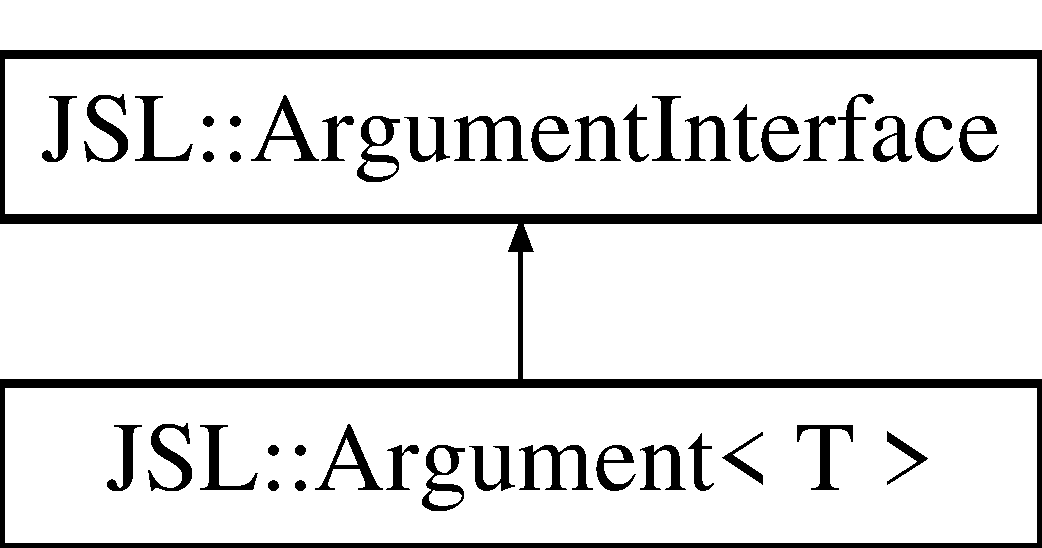
\includegraphics[height=2.000000cm]{classJSL_1_1Argument}
\end{center}
\end{figure}
\subsection*{Public Member Functions}
\begin{DoxyCompactItemize}
\item 
\hyperlink{classJSL_1_1Argument_ab438509a3c030516de72f3f493295bd5}{Argument} ()
\begin{DoxyCompactList}\small\item\em Default constructor. \end{DoxyCompactList}\item 
\hyperlink{classJSL_1_1Argument_ab07e7981db832cce30f534c67f6491f4}{Argument} (std\+::string trigger)
\begin{DoxyCompactList}\small\item\em Constructor initialising the \hyperlink{classJSL_1_1ArgumentInterface_afa2d1f96c4971070d3de5824f297312f}{Trigger\+String}. Value is set to uninitialised memory of the Template type. \end{DoxyCompactList}\item 
\hyperlink{classJSL_1_1Argument_a2511f7c98ee2b0b59650f468341b8747}{Argument} (T default\+Value, std\+::string trigger)
\begin{DoxyCompactList}\small\item\em Constructor which initialises the \hyperlink{classJSL_1_1ArgumentInterface_afa2d1f96c4971070d3de5824f297312f}{Trigger\+String} and \hyperlink{classJSL_1_1Argument_a83ada5bfa412192f76dd4290f679defd}{Value} members. \end{DoxyCompactList}\item 
\hyperlink{classJSL_1_1Argument_a4d187d2fb658021866b173987b920ab4}{Argument} (T default\+Value, std\+::string trigger, int argc, char $\ast$argv\mbox{[}$\,$\mbox{]})
\begin{DoxyCompactList}\small\item\em Constructor which initialises as per \hyperlink{classJSL_1_1Argument_a2511f7c98ee2b0b59650f468341b8747}{Argument(\+T default\+Value, std\+::string trigger)}, but which also immediately calls \hyperlink{classJSL_1_1Argument_aa2b18bb35e90f91e224a06d60835053a}{List\+Parse()} to check for assignment. \end{DoxyCompactList}\item 
\hyperlink{classJSL_1_1Argument_a83799e9089f88d7e6cf30990fae42610}{Argument} (T default\+Value, std\+::string trigger, std\+::string config\+File, char config\+Delimiter)
\begin{DoxyCompactList}\small\item\em Constructor which initialises as per \hyperlink{classJSL_1_1Argument_a2511f7c98ee2b0b59650f468341b8747}{Argument(\+T default\+Value, std\+::string trigger)}, but which also immediately calls \hyperlink{classJSL_1_1Argument_aa626ff37dbebaf0501614dc625a76383}{Configure()} to check for assignment. \end{DoxyCompactList}\item 
void \hyperlink{classJSL_1_1Argument_aa626ff37dbebaf0501614dc625a76383}{Configure} (std\+::string config\+File, char config\+Delimiter)
\begin{DoxyCompactList}\small\item\em Iterate through a configuration file, extracting Name/\+Value pairs and calling \hyperlink{classJSL_1_1Argument_a8984e7ce23155259d90a3e98170f36e0}{Parse()} in them. Each Name/\+Value pair should be on a new line in the file, and separated by the {\itshape config\+Delimiter}. \end{DoxyCompactList}\item 
void \hyperlink{classJSL_1_1Argument_aa2b18bb35e90f91e224a06d60835053a}{List\+Parse} (int argc, char $\ast$argv\mbox{[}$\,$\mbox{]})
\begin{DoxyCompactList}\small\item\em Iterate through the provided commandline args, extracting Name/\+Value pairs and calling \hyperlink{classJSL_1_1Argument_a8984e7ce23155259d90a3e98170f36e0}{Parse()} on them. \end{DoxyCompactList}\item 
void \hyperlink{classJSL_1_1Argument_a8984e7ce23155259d90a3e98170f36e0}{Parse} (char $\ast$name, char $\ast$value)
\begin{DoxyCompactList}\small\item\em Checks if the Name matches the Trigger\+String. For a successful match, Name must be prefaced by one more dash than found in Trigger\+String. \end{DoxyCompactList}\item 
\hyperlink{classJSL_1_1Argument_a965bc0dfdce6e03380605af313f8c880}{operator T} ()
\begin{DoxyCompactList}\small\item\em Allow the \hyperlink{classJSL_1_1Argument}{Argument} object to be implicitly casted into the value of \hyperlink{classJSL_1_1Argument_a83ada5bfa412192f76dd4290f679defd}{Value}, and hence treated as an object of the templated type. \end{DoxyCompactList}\end{DoxyCompactItemize}
\subsection*{Data Fields}
\begin{DoxyCompactItemize}
\item 
T \hyperlink{classJSL_1_1Argument_a83ada5bfa412192f76dd4290f679defd}{Value}
\begin{DoxyCompactList}\small\item\em The current value of the argument. \end{DoxyCompactList}\end{DoxyCompactItemize}
\subsection*{Private Member Functions}
\begin{DoxyCompactItemize}
\item 
void \hyperlink{classJSL_1_1Argument_a8614eb66f807132c4323847e05e666c4}{Check\+For\+Invalid\+Triggers} ()
\begin{DoxyCompactList}\small\item\em Some Triggers are disallowed -\/ they usually are protected names such as \char`\"{}help\char`\"{}, though other properties may trigger this funciton to throw an error. \end{DoxyCompactList}\item 
virtual void \hyperlink{classJSL_1_1Argument_abc43696d406a6d369cd1b3d8cb1540b5}{Assign\+Value} (char $\ast$value)
\begin{DoxyCompactList}\small\item\em Virtual override for template-\/specific Assign\+Value calls. Most template types will require a custom handler to convert value into the chosen template type -- some default ones are provided below. \end{DoxyCompactList}\item 
void \hyperlink{classJSL_1_1Argument_af0c053ad614c0f20c48cf31389eee7e9}{Assign\+Value} (std\+::string value)
\begin{DoxyCompactList}\small\item\em Allow value assignments with strings, because C++ char/strings made my head hurt. \end{DoxyCompactList}\item 
{\footnotesize template$<$$>$ }\\void \hyperlink{classJSL_1_1Argument_a2b60a11be4f0ba28dfb3395c49ced06b}{Assign\+Value} (char $\ast$value)
\begin{DoxyCompactList}\small\item\em Override of the \hyperlink{classJSL_1_1Argument_abc43696d406a6d369cd1b3d8cb1540b5}{Assign\+Value()} function for Argument$<$double$>$ objects. Throws an error if the value is a non-\/integer, to prevent silent casting/truncation. \end{DoxyCompactList}\item 
{\footnotesize template$<$$>$ }\\void \hyperlink{classJSL_1_1Argument_afbd6b9b5c50de60cee39f4b0ab327375}{Assign\+Value} (char $\ast$value)
\begin{DoxyCompactList}\small\item\em Override of the \hyperlink{classJSL_1_1Argument_abc43696d406a6d369cd1b3d8cb1540b5}{Assign\+Value()} function for Argument$<$double$>$ objects. \end{DoxyCompactList}\item 
{\footnotesize template$<$$>$ }\\void \hyperlink{classJSL_1_1Argument_a1b443f8b8948e7aaec2154ed15e6f08f}{Assign\+Value} (char $\ast$value)
\begin{DoxyCompactList}\small\item\em Override of the \hyperlink{classJSL_1_1Argument_abc43696d406a6d369cd1b3d8cb1540b5}{Assign\+Value()} function for \hyperlink{classJSL_1_1Argument_ab438509a3c030516de72f3f493295bd5}{Argument$<$std\+::string$>$} objects. \end{DoxyCompactList}\item 
{\footnotesize template$<$$>$ }\\void \hyperlink{classJSL_1_1Argument_ac71e37555de1dea3b6d297bf0909a920}{Assign\+Value} (char $\ast$value)
\begin{DoxyCompactList}\small\item\em Override of the \hyperlink{classJSL_1_1Argument_abc43696d406a6d369cd1b3d8cb1540b5}{Assign\+Value()} function for Argument$<$bool$>$ objects. Accepts only 0/1 as valid bool-\/strings. \end{DoxyCompactList}\end{DoxyCompactItemize}
\subsection*{Additional Inherited Members}


\subsection{Detailed Description}
\subsubsection*{template$<$class T$>$\newline
class J\+S\+L\+::\+Argument$<$ T $>$}

A class which allows arbitrary template parameters to be read in as command-\/line arguments using a Name/\+Value pair system. Upon construction, the \hyperlink{classJSL_1_1Argument_a83ada5bfa412192f76dd4290f679defd}{Value} parameter takes the default value (if provided), until it is overriden by a successful argument/\hyperlink{classJSL_1_1ArgumentInterface_afa2d1f96c4971070d3de5824f297312f}{Trigger\+String} match. 

\subsection{Constructor \& Destructor Documentation}
\mbox{\Hypertarget{classJSL_1_1Argument_ab438509a3c030516de72f3f493295bd5}\label{classJSL_1_1Argument_ab438509a3c030516de72f3f493295bd5}} 
\index{J\+S\+L\+::\+Argument@{J\+S\+L\+::\+Argument}!Argument@{Argument}}
\index{Argument@{Argument}!J\+S\+L\+::\+Argument@{J\+S\+L\+::\+Argument}}
\subsubsection{\texorpdfstring{Argument()}{Argument()}\hspace{0.1cm}{\footnotesize\ttfamily [1/5]}}
{\footnotesize\ttfamily template$<$class T $>$ \\
\hyperlink{classJSL_1_1Argument}{J\+S\+L\+::\+Argument}$<$ T $>$\+::\hyperlink{classJSL_1_1Argument}{Argument} (\begin{DoxyParamCaption}{ }\end{DoxyParamCaption})\hspace{0.3cm}{\ttfamily [inline]}}



Default constructor. 

\mbox{\Hypertarget{classJSL_1_1Argument_ab07e7981db832cce30f534c67f6491f4}\label{classJSL_1_1Argument_ab07e7981db832cce30f534c67f6491f4}} 
\index{J\+S\+L\+::\+Argument@{J\+S\+L\+::\+Argument}!Argument@{Argument}}
\index{Argument@{Argument}!J\+S\+L\+::\+Argument@{J\+S\+L\+::\+Argument}}
\subsubsection{\texorpdfstring{Argument()}{Argument()}\hspace{0.1cm}{\footnotesize\ttfamily [2/5]}}
{\footnotesize\ttfamily template$<$class T $>$ \\
\hyperlink{classJSL_1_1Argument}{J\+S\+L\+::\+Argument}$<$ T $>$\+::\hyperlink{classJSL_1_1Argument}{Argument} (\begin{DoxyParamCaption}\item[{std\+::string}]{trigger }\end{DoxyParamCaption})\hspace{0.3cm}{\ttfamily [inline]}}



Constructor initialising the \hyperlink{classJSL_1_1ArgumentInterface_afa2d1f96c4971070d3de5824f297312f}{Trigger\+String}. Value is set to uninitialised memory of the Template type. 


\begin{DoxyParams}{Parameters}
{\em trigger} & The value of \hyperlink{classJSL_1_1ArgumentInterface_afa2d1f96c4971070d3de5824f297312f}{Trigger\+String}, and the \char`\"{}name\char`\"{} of this parameter \\
\hline
\end{DoxyParams}
\mbox{\Hypertarget{classJSL_1_1Argument_a2511f7c98ee2b0b59650f468341b8747}\label{classJSL_1_1Argument_a2511f7c98ee2b0b59650f468341b8747}} 
\index{J\+S\+L\+::\+Argument@{J\+S\+L\+::\+Argument}!Argument@{Argument}}
\index{Argument@{Argument}!J\+S\+L\+::\+Argument@{J\+S\+L\+::\+Argument}}
\subsubsection{\texorpdfstring{Argument()}{Argument()}\hspace{0.1cm}{\footnotesize\ttfamily [3/5]}}
{\footnotesize\ttfamily template$<$class T $>$ \\
\hyperlink{classJSL_1_1Argument}{J\+S\+L\+::\+Argument}$<$ T $>$\+::\hyperlink{classJSL_1_1Argument}{Argument} (\begin{DoxyParamCaption}\item[{T}]{default\+Value,  }\item[{std\+::string}]{trigger }\end{DoxyParamCaption})\hspace{0.3cm}{\ttfamily [inline]}}



Constructor which initialises the \hyperlink{classJSL_1_1ArgumentInterface_afa2d1f96c4971070d3de5824f297312f}{Trigger\+String} and \hyperlink{classJSL_1_1Argument_a83ada5bfa412192f76dd4290f679defd}{Value} members. 


\begin{DoxyParams}{Parameters}
{\em default\+Value} & The initialisation value of \hyperlink{classJSL_1_1Argument_a83ada5bfa412192f76dd4290f679defd}{Value} -\/ overridden if \hyperlink{classJSL_1_1Argument_a8984e7ce23155259d90a3e98170f36e0}{Parse()} is called. \\
\hline
{\em trigger} & The value of \hyperlink{classJSL_1_1ArgumentInterface_afa2d1f96c4971070d3de5824f297312f}{Trigger\+String}, and the \char`\"{}name\char`\"{} of this parameter \\
\hline
\end{DoxyParams}
\mbox{\Hypertarget{classJSL_1_1Argument_a4d187d2fb658021866b173987b920ab4}\label{classJSL_1_1Argument_a4d187d2fb658021866b173987b920ab4}} 
\index{J\+S\+L\+::\+Argument@{J\+S\+L\+::\+Argument}!Argument@{Argument}}
\index{Argument@{Argument}!J\+S\+L\+::\+Argument@{J\+S\+L\+::\+Argument}}
\subsubsection{\texorpdfstring{Argument()}{Argument()}\hspace{0.1cm}{\footnotesize\ttfamily [4/5]}}
{\footnotesize\ttfamily template$<$class T $>$ \\
\hyperlink{classJSL_1_1Argument}{J\+S\+L\+::\+Argument}$<$ T $>$\+::\hyperlink{classJSL_1_1Argument}{Argument} (\begin{DoxyParamCaption}\item[{T}]{default\+Value,  }\item[{std\+::string}]{trigger,  }\item[{int}]{argc,  }\item[{char $\ast$}]{argv\mbox{[}$\,$\mbox{]} }\end{DoxyParamCaption})\hspace{0.3cm}{\ttfamily [inline]}}



Constructor which initialises as per \hyperlink{classJSL_1_1Argument_a2511f7c98ee2b0b59650f468341b8747}{Argument(\+T default\+Value, std\+::string trigger)}, but which also immediately calls \hyperlink{classJSL_1_1Argument_aa2b18bb35e90f91e224a06d60835053a}{List\+Parse()} to check for assignment. 


\begin{DoxyParams}{Parameters}
{\em default\+Value} & The initialisation value of \hyperlink{classJSL_1_1Argument_a83ada5bfa412192f76dd4290f679defd}{Value} -\/ overridden if \hyperlink{classJSL_1_1Argument_a8984e7ce23155259d90a3e98170f36e0}{Parse()} is called. \\
\hline
{\em trigger} & The value of \hyperlink{classJSL_1_1ArgumentInterface_afa2d1f96c4971070d3de5824f297312f}{Trigger\+String}, and the \char`\"{}name\char`\"{} of this parameter \\
\hline
{\em argc} & The number of commandline arguments \\
\hline
{\em argv\mbox{[}$\,$\mbox{]}} & the command line list \\
\hline
\end{DoxyParams}
\mbox{\Hypertarget{classJSL_1_1Argument_a83799e9089f88d7e6cf30990fae42610}\label{classJSL_1_1Argument_a83799e9089f88d7e6cf30990fae42610}} 
\index{J\+S\+L\+::\+Argument@{J\+S\+L\+::\+Argument}!Argument@{Argument}}
\index{Argument@{Argument}!J\+S\+L\+::\+Argument@{J\+S\+L\+::\+Argument}}
\subsubsection{\texorpdfstring{Argument()}{Argument()}\hspace{0.1cm}{\footnotesize\ttfamily [5/5]}}
{\footnotesize\ttfamily template$<$class T $>$ \\
\hyperlink{classJSL_1_1Argument}{J\+S\+L\+::\+Argument}$<$ T $>$\+::\hyperlink{classJSL_1_1Argument}{Argument} (\begin{DoxyParamCaption}\item[{T}]{default\+Value,  }\item[{std\+::string}]{trigger,  }\item[{std\+::string}]{config\+File,  }\item[{char}]{config\+Delimiter }\end{DoxyParamCaption})\hspace{0.3cm}{\ttfamily [inline]}}



Constructor which initialises as per \hyperlink{classJSL_1_1Argument_a2511f7c98ee2b0b59650f468341b8747}{Argument(\+T default\+Value, std\+::string trigger)}, but which also immediately calls \hyperlink{classJSL_1_1Argument_aa626ff37dbebaf0501614dc625a76383}{Configure()} to check for assignment. 


\begin{DoxyParams}{Parameters}
{\em default\+Value} & The initialisation value of \hyperlink{classJSL_1_1Argument_a83ada5bfa412192f76dd4290f679defd}{Value} -\/ overridden if \hyperlink{classJSL_1_1Argument_a8984e7ce23155259d90a3e98170f36e0}{Parse()} is called. \\
\hline
{\em trigger} & The value of \hyperlink{classJSL_1_1ArgumentInterface_afa2d1f96c4971070d3de5824f297312f}{Trigger\+String}, and the \char`\"{}name\char`\"{} of this parameter \\
\hline
{\em config\+File} & The path to the file to open and parse for configuration data \\
\hline
{\em config\+Delimiter} & The delimiter used to separate Name/\+Value pairs in the cofiguration file \\
\hline
\end{DoxyParams}


\subsection{Member Function Documentation}
\mbox{\Hypertarget{classJSL_1_1Argument_abc43696d406a6d369cd1b3d8cb1540b5}\label{classJSL_1_1Argument_abc43696d406a6d369cd1b3d8cb1540b5}} 
\index{J\+S\+L\+::\+Argument@{J\+S\+L\+::\+Argument}!Assign\+Value@{Assign\+Value}}
\index{Assign\+Value@{Assign\+Value}!J\+S\+L\+::\+Argument@{J\+S\+L\+::\+Argument}}
\subsubsection{\texorpdfstring{Assign\+Value()}{AssignValue()}\hspace{0.1cm}{\footnotesize\ttfamily [1/6]}}
{\footnotesize\ttfamily template$<$class T $>$ \\
virtual void \hyperlink{classJSL_1_1Argument}{J\+S\+L\+::\+Argument}$<$ T $>$\+::Assign\+Value (\begin{DoxyParamCaption}\item[{char $\ast$}]{value }\end{DoxyParamCaption})\hspace{0.3cm}{\ttfamily [inline]}, {\ttfamily [private]}, {\ttfamily [virtual]}}



Virtual override for template-\/specific Assign\+Value calls. Most template types will require a custom handler to convert value into the chosen template type -- some default ones are provided below. 

\mbox{\Hypertarget{classJSL_1_1Argument_af0c053ad614c0f20c48cf31389eee7e9}\label{classJSL_1_1Argument_af0c053ad614c0f20c48cf31389eee7e9}} 
\index{J\+S\+L\+::\+Argument@{J\+S\+L\+::\+Argument}!Assign\+Value@{Assign\+Value}}
\index{Assign\+Value@{Assign\+Value}!J\+S\+L\+::\+Argument@{J\+S\+L\+::\+Argument}}
\subsubsection{\texorpdfstring{Assign\+Value()}{AssignValue()}\hspace{0.1cm}{\footnotesize\ttfamily [2/6]}}
{\footnotesize\ttfamily template$<$class T $>$ \\
void \hyperlink{classJSL_1_1Argument}{J\+S\+L\+::\+Argument}$<$ T $>$\+::Assign\+Value (\begin{DoxyParamCaption}\item[{std\+::string}]{value }\end{DoxyParamCaption})\hspace{0.3cm}{\ttfamily [inline]}, {\ttfamily [private]}}



Allow value assignments with strings, because C++ char/strings made my head hurt. 

\mbox{\Hypertarget{classJSL_1_1Argument_a2b60a11be4f0ba28dfb3395c49ced06b}\label{classJSL_1_1Argument_a2b60a11be4f0ba28dfb3395c49ced06b}} 
\index{J\+S\+L\+::\+Argument@{J\+S\+L\+::\+Argument}!Assign\+Value@{Assign\+Value}}
\index{Assign\+Value@{Assign\+Value}!J\+S\+L\+::\+Argument@{J\+S\+L\+::\+Argument}}
\subsubsection{\texorpdfstring{Assign\+Value()}{AssignValue()}\hspace{0.1cm}{\footnotesize\ttfamily [3/6]}}
{\footnotesize\ttfamily template$<$$>$ \\
void \hyperlink{classJSL_1_1Argument}{J\+S\+L\+::\+Argument}$<$ int $>$\+::Assign\+Value (\begin{DoxyParamCaption}\item[{char $\ast$}]{value }\end{DoxyParamCaption})\hspace{0.3cm}{\ttfamily [inline]}, {\ttfamily [private]}}



Override of the \hyperlink{classJSL_1_1Argument_abc43696d406a6d369cd1b3d8cb1540b5}{Assign\+Value()} function for Argument$<$double$>$ objects. Throws an error if the value is a non-\/integer, to prevent silent casting/truncation. 

\mbox{\Hypertarget{classJSL_1_1Argument_afbd6b9b5c50de60cee39f4b0ab327375}\label{classJSL_1_1Argument_afbd6b9b5c50de60cee39f4b0ab327375}} 
\index{J\+S\+L\+::\+Argument@{J\+S\+L\+::\+Argument}!Assign\+Value@{Assign\+Value}}
\index{Assign\+Value@{Assign\+Value}!J\+S\+L\+::\+Argument@{J\+S\+L\+::\+Argument}}
\subsubsection{\texorpdfstring{Assign\+Value()}{AssignValue()}\hspace{0.1cm}{\footnotesize\ttfamily [4/6]}}
{\footnotesize\ttfamily template$<$$>$ \\
void \hyperlink{classJSL_1_1Argument}{J\+S\+L\+::\+Argument}$<$ double $>$\+::Assign\+Value (\begin{DoxyParamCaption}\item[{char $\ast$}]{value }\end{DoxyParamCaption})\hspace{0.3cm}{\ttfamily [inline]}, {\ttfamily [private]}}



Override of the \hyperlink{classJSL_1_1Argument_abc43696d406a6d369cd1b3d8cb1540b5}{Assign\+Value()} function for Argument$<$double$>$ objects. 

\mbox{\Hypertarget{classJSL_1_1Argument_a1b443f8b8948e7aaec2154ed15e6f08f}\label{classJSL_1_1Argument_a1b443f8b8948e7aaec2154ed15e6f08f}} 
\index{J\+S\+L\+::\+Argument@{J\+S\+L\+::\+Argument}!Assign\+Value@{Assign\+Value}}
\index{Assign\+Value@{Assign\+Value}!J\+S\+L\+::\+Argument@{J\+S\+L\+::\+Argument}}
\subsubsection{\texorpdfstring{Assign\+Value()}{AssignValue()}\hspace{0.1cm}{\footnotesize\ttfamily [5/6]}}
{\footnotesize\ttfamily template$<$$>$ \\
void \hyperlink{classJSL_1_1Argument}{J\+S\+L\+::\+Argument}$<$ std\+::string $>$\+::Assign\+Value (\begin{DoxyParamCaption}\item[{char $\ast$}]{value }\end{DoxyParamCaption})\hspace{0.3cm}{\ttfamily [inline]}, {\ttfamily [private]}}



Override of the \hyperlink{classJSL_1_1Argument_abc43696d406a6d369cd1b3d8cb1540b5}{Assign\+Value()} function for \hyperlink{classJSL_1_1Argument_ab438509a3c030516de72f3f493295bd5}{Argument$<$std\+::string$>$} objects. 

\mbox{\Hypertarget{classJSL_1_1Argument_ac71e37555de1dea3b6d297bf0909a920}\label{classJSL_1_1Argument_ac71e37555de1dea3b6d297bf0909a920}} 
\index{J\+S\+L\+::\+Argument@{J\+S\+L\+::\+Argument}!Assign\+Value@{Assign\+Value}}
\index{Assign\+Value@{Assign\+Value}!J\+S\+L\+::\+Argument@{J\+S\+L\+::\+Argument}}
\subsubsection{\texorpdfstring{Assign\+Value()}{AssignValue()}\hspace{0.1cm}{\footnotesize\ttfamily [6/6]}}
{\footnotesize\ttfamily template$<$$>$ \\
void \hyperlink{classJSL_1_1Argument}{J\+S\+L\+::\+Argument}$<$ bool $>$\+::Assign\+Value (\begin{DoxyParamCaption}\item[{char $\ast$}]{value }\end{DoxyParamCaption})\hspace{0.3cm}{\ttfamily [inline]}, {\ttfamily [private]}}



Override of the \hyperlink{classJSL_1_1Argument_abc43696d406a6d369cd1b3d8cb1540b5}{Assign\+Value()} function for Argument$<$bool$>$ objects. Accepts only 0/1 as valid bool-\/strings. 

\mbox{\Hypertarget{classJSL_1_1Argument_a8614eb66f807132c4323847e05e666c4}\label{classJSL_1_1Argument_a8614eb66f807132c4323847e05e666c4}} 
\index{J\+S\+L\+::\+Argument@{J\+S\+L\+::\+Argument}!Check\+For\+Invalid\+Triggers@{Check\+For\+Invalid\+Triggers}}
\index{Check\+For\+Invalid\+Triggers@{Check\+For\+Invalid\+Triggers}!J\+S\+L\+::\+Argument@{J\+S\+L\+::\+Argument}}
\subsubsection{\texorpdfstring{Check\+For\+Invalid\+Triggers()}{CheckForInvalidTriggers()}}
{\footnotesize\ttfamily template$<$class T $>$ \\
void \hyperlink{classJSL_1_1Argument}{J\+S\+L\+::\+Argument}$<$ T $>$\+::Check\+For\+Invalid\+Triggers (\begin{DoxyParamCaption}{ }\end{DoxyParamCaption})\hspace{0.3cm}{\ttfamily [inline]}, {\ttfamily [private]}}



Some Triggers are disallowed -\/ they usually are protected names such as \char`\"{}help\char`\"{}, though other properties may trigger this funciton to throw an error. 

\mbox{\Hypertarget{classJSL_1_1Argument_aa626ff37dbebaf0501614dc625a76383}\label{classJSL_1_1Argument_aa626ff37dbebaf0501614dc625a76383}} 
\index{J\+S\+L\+::\+Argument@{J\+S\+L\+::\+Argument}!Configure@{Configure}}
\index{Configure@{Configure}!J\+S\+L\+::\+Argument@{J\+S\+L\+::\+Argument}}
\subsubsection{\texorpdfstring{Configure()}{Configure()}}
{\footnotesize\ttfamily template$<$class T $>$ \\
void \hyperlink{classJSL_1_1Argument}{J\+S\+L\+::\+Argument}$<$ T $>$\+::Configure (\begin{DoxyParamCaption}\item[{std\+::string}]{config\+File,  }\item[{char}]{config\+Delimiter }\end{DoxyParamCaption})\hspace{0.3cm}{\ttfamily [inline]}, {\ttfamily [virtual]}}



Iterate through a configuration file, extracting Name/\+Value pairs and calling \hyperlink{classJSL_1_1Argument_a8984e7ce23155259d90a3e98170f36e0}{Parse()} in them. Each Name/\+Value pair should be on a new line in the file, and separated by the {\itshape config\+Delimiter}. 


\begin{DoxyParams}{Parameters}
{\em config\+File} & The path to the file to open and parse for configuration data \\
\hline
{\em config\+Delimiter} & The delimiter used to separate Name/\+Value pairs in the cofiguration file \\
\hline
\end{DoxyParams}


Reimplemented from \hyperlink{classJSL_1_1ArgumentInterface_aac7c3106f99c407e625b9bc6a6c8c446}{J\+S\+L\+::\+Argument\+Interface}.

\mbox{\Hypertarget{classJSL_1_1Argument_aa2b18bb35e90f91e224a06d60835053a}\label{classJSL_1_1Argument_aa2b18bb35e90f91e224a06d60835053a}} 
\index{J\+S\+L\+::\+Argument@{J\+S\+L\+::\+Argument}!List\+Parse@{List\+Parse}}
\index{List\+Parse@{List\+Parse}!J\+S\+L\+::\+Argument@{J\+S\+L\+::\+Argument}}
\subsubsection{\texorpdfstring{List\+Parse()}{ListParse()}}
{\footnotesize\ttfamily template$<$class T $>$ \\
void \hyperlink{classJSL_1_1Argument}{J\+S\+L\+::\+Argument}$<$ T $>$\+::List\+Parse (\begin{DoxyParamCaption}\item[{int}]{argc,  }\item[{char $\ast$}]{argv\mbox{[}$\,$\mbox{]} }\end{DoxyParamCaption})\hspace{0.3cm}{\ttfamily [inline]}, {\ttfamily [virtual]}}



Iterate through the provided commandline args, extracting Name/\+Value pairs and calling \hyperlink{classJSL_1_1Argument_a8984e7ce23155259d90a3e98170f36e0}{Parse()} on them. 


\begin{DoxyParams}{Parameters}
{\em argc} & The number of arguments passed to the program \\
\hline
{\em argv\mbox{[}$\,$\mbox{]}} & The argument list (argv\mbox{[}0\mbox{]} is assumed to be the the name of the program, and is ignored) \\
\hline
\end{DoxyParams}


Reimplemented from \hyperlink{classJSL_1_1ArgumentInterface_a256b5bd88b5f6638353f108c48f3ee65}{J\+S\+L\+::\+Argument\+Interface}.

\mbox{\Hypertarget{classJSL_1_1Argument_a965bc0dfdce6e03380605af313f8c880}\label{classJSL_1_1Argument_a965bc0dfdce6e03380605af313f8c880}} 
\index{J\+S\+L\+::\+Argument@{J\+S\+L\+::\+Argument}!operator T@{operator T}}
\index{operator T@{operator T}!J\+S\+L\+::\+Argument@{J\+S\+L\+::\+Argument}}
\subsubsection{\texorpdfstring{operator T()}{operator T()}}
{\footnotesize\ttfamily template$<$class T $>$ \\
\hyperlink{classJSL_1_1Argument}{J\+S\+L\+::\+Argument}$<$ T $>$\+::operator T (\begin{DoxyParamCaption}{ }\end{DoxyParamCaption})\hspace{0.3cm}{\ttfamily [inline]}}



Allow the \hyperlink{classJSL_1_1Argument}{Argument} object to be implicitly casted into the value of \hyperlink{classJSL_1_1Argument_a83ada5bfa412192f76dd4290f679defd}{Value}, and hence treated as an object of the templated type. 

\mbox{\Hypertarget{classJSL_1_1Argument_a8984e7ce23155259d90a3e98170f36e0}\label{classJSL_1_1Argument_a8984e7ce23155259d90a3e98170f36e0}} 
\index{J\+S\+L\+::\+Argument@{J\+S\+L\+::\+Argument}!Parse@{Parse}}
\index{Parse@{Parse}!J\+S\+L\+::\+Argument@{J\+S\+L\+::\+Argument}}
\subsubsection{\texorpdfstring{Parse()}{Parse()}}
{\footnotesize\ttfamily template$<$class T $>$ \\
void \hyperlink{classJSL_1_1Argument}{J\+S\+L\+::\+Argument}$<$ T $>$\+::Parse (\begin{DoxyParamCaption}\item[{char $\ast$}]{name,  }\item[{char $\ast$}]{value }\end{DoxyParamCaption})\hspace{0.3cm}{\ttfamily [inline]}, {\ttfamily [virtual]}}



Checks if the Name matches the Trigger\+String. For a successful match, Name must be prefaced by one more dash than found in Trigger\+String. 


\begin{DoxyParams}{Parameters}
{\em name} & The name-\/string of the Name/\+Value pair\\
\hline
{\em value} & The value-\/string of the Name/\+Value pair. \\
\hline
\end{DoxyParams}


Reimplemented from \hyperlink{classJSL_1_1ArgumentInterface_a28b487f7a4fa6e721ed6629abe2073f2}{J\+S\+L\+::\+Argument\+Interface}.



\subsection{Field Documentation}
\mbox{\Hypertarget{classJSL_1_1Argument_a83ada5bfa412192f76dd4290f679defd}\label{classJSL_1_1Argument_a83ada5bfa412192f76dd4290f679defd}} 
\index{J\+S\+L\+::\+Argument@{J\+S\+L\+::\+Argument}!Value@{Value}}
\index{Value@{Value}!J\+S\+L\+::\+Argument@{J\+S\+L\+::\+Argument}}
\subsubsection{\texorpdfstring{Value}{Value}}
{\footnotesize\ttfamily template$<$class T $>$ \\
T \hyperlink{classJSL_1_1Argument}{J\+S\+L\+::\+Argument}$<$ T $>$\+::Value}



The current value of the argument. 



The documentation for this class was generated from the following file\+:\begin{DoxyCompactItemize}
\item 
/home/fraserj/\+Documents/\+Work/\+J\+S\+L/\+Command\+Args/\hyperlink{Argument_8h}{Argument.\+h}\end{DoxyCompactItemize}

\hypertarget{classJSL_1_1ArgumentInterface}{}\doxysection{J\+SL\+::Argument\+Interface Class Reference}
\label{classJSL_1_1ArgumentInterface}\index{JSL::ArgumentInterface@{JSL::ArgumentInterface}}


{\ttfamily \#include $<$Argument.\+h$>$}

Inheritance diagram for J\+SL\+::Argument\+Interface\+:\begin{figure}[H]
\begin{center}
\leavevmode
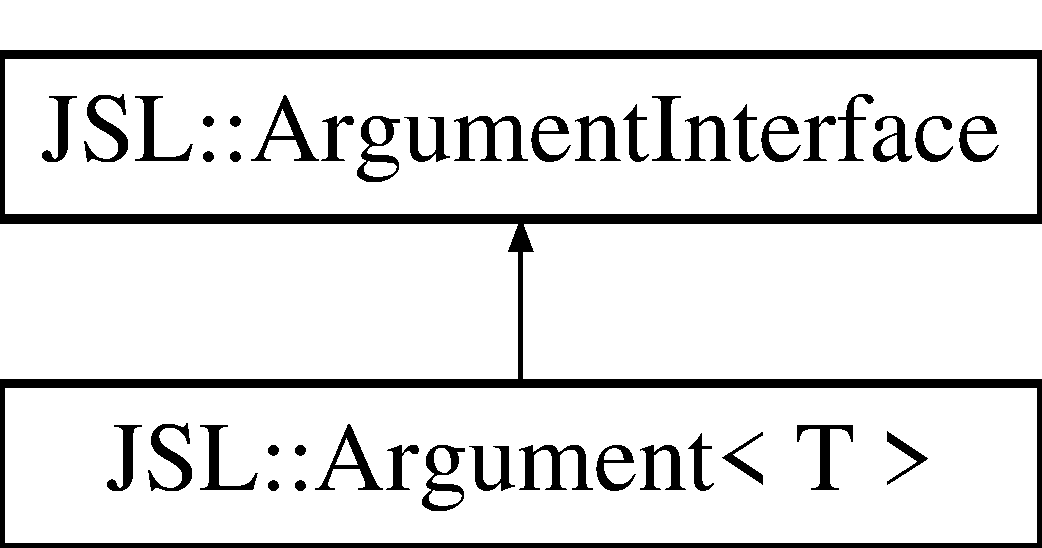
\includegraphics[height=2.000000cm]{classJSL_1_1ArgumentInterface}
\end{center}
\end{figure}
\doxysubsection*{Public Member Functions}
\begin{DoxyCompactItemize}
\item 
virtual void \mbox{\hyperlink{classJSL_1_1ArgumentInterface_a28b487f7a4fa6e721ed6629abe2073f2}{Parse}} (char $\ast$name, char $\ast$value)
\begin{DoxyCompactList}\small\item\em Virtual alias for \mbox{\hyperlink{classJSL_1_1Argument_a8984e7ce23155259d90a3e98170f36e0}{Argument\+::\+Parse()}} \end{DoxyCompactList}\item 
virtual void \mbox{\hyperlink{classJSL_1_1ArgumentInterface_a256b5bd88b5f6638353f108c48f3ee65}{List\+Parse}} (int argc, char $\ast$argv\mbox{[}$\,$\mbox{]})
\begin{DoxyCompactList}\small\item\em Virtual alias for \mbox{\hyperlink{classJSL_1_1Argument_aa2b18bb35e90f91e224a06d60835053a}{Argument\+::\+List\+Parse()}} \end{DoxyCompactList}\item 
virtual void \mbox{\hyperlink{classJSL_1_1ArgumentInterface_aac7c3106f99c407e625b9bc6a6c8c446}{Configure}} (std\+::string config\+File, char config\+Delimiter)
\begin{DoxyCompactList}\small\item\em Virtual alias for \mbox{\hyperlink{classJSL_1_1Argument_aa626ff37dbebaf0501614dc625a76383}{Argument\+::\+Configure()}} \end{DoxyCompactList}\end{DoxyCompactItemize}
\doxysubsection*{Protected Attributes}
\begin{DoxyCompactItemize}
\item 
std\+::string \mbox{\hyperlink{classJSL_1_1ArgumentInterface_afa2d1f96c4971070d3de5824f297312f}{Trigger\+String}}
\begin{DoxyCompactList}\small\item\em The chosen \char`\"{}\+Name\char`\"{} of the \mbox{\hyperlink{classJSL_1_1Argument}{Argument}} -\/ the string which will trigger the \mbox{\hyperlink{classJSL_1_1ArgumentInterface_a28b487f7a4fa6e721ed6629abe2073f2}{Parse()}} function to write in the passed value. \end{DoxyCompactList}\end{DoxyCompactItemize}


\doxysubsection{Detailed Description}
A wrapper class for all \mbox{\hyperlink{classJSL_1_1Argument}{Argument}} objects, enabling heterogenous argument lists etc. to be constructed. ~\newline
 Contains the virtual methods common to all objects. All \mbox{\hyperlink{classJSL_1_1Argument}{Argument}} objects are assumed to take name-\/value pairs, with the associated name indicated by the \mbox{\hyperlink{classJSL_1_1ArgumentInterface_afa2d1f96c4971070d3de5824f297312f}{Trigger\+String}} 

\doxysubsection{Member Function Documentation}
\mbox{\Hypertarget{classJSL_1_1ArgumentInterface_aac7c3106f99c407e625b9bc6a6c8c446}\label{classJSL_1_1ArgumentInterface_aac7c3106f99c407e625b9bc6a6c8c446}} 
\index{JSL::ArgumentInterface@{JSL::ArgumentInterface}!Configure@{Configure}}
\index{Configure@{Configure}!JSL::ArgumentInterface@{JSL::ArgumentInterface}}
\doxysubsubsection{\texorpdfstring{Configure()}{Configure()}}
{\footnotesize\ttfamily virtual void J\+S\+L\+::\+Argument\+Interface\+::\+Configure (\begin{DoxyParamCaption}\item[{std\+::string}]{config\+File,  }\item[{char}]{config\+Delimiter }\end{DoxyParamCaption})\hspace{0.3cm}{\ttfamily [inline]}, {\ttfamily [virtual]}}



Virtual alias for \mbox{\hyperlink{classJSL_1_1Argument_aa626ff37dbebaf0501614dc625a76383}{Argument\+::\+Configure()}} 



Reimplemented in \mbox{\hyperlink{classJSL_1_1Argument_aa626ff37dbebaf0501614dc625a76383}{J\+S\+L\+::\+Argument$<$ T $>$}}.

\mbox{\Hypertarget{classJSL_1_1ArgumentInterface_a256b5bd88b5f6638353f108c48f3ee65}\label{classJSL_1_1ArgumentInterface_a256b5bd88b5f6638353f108c48f3ee65}} 
\index{JSL::ArgumentInterface@{JSL::ArgumentInterface}!ListParse@{ListParse}}
\index{ListParse@{ListParse}!JSL::ArgumentInterface@{JSL::ArgumentInterface}}
\doxysubsubsection{\texorpdfstring{ListParse()}{ListParse()}}
{\footnotesize\ttfamily virtual void J\+S\+L\+::\+Argument\+Interface\+::\+List\+Parse (\begin{DoxyParamCaption}\item[{int}]{argc,  }\item[{char $\ast$}]{argv\mbox{[}$\,$\mbox{]} }\end{DoxyParamCaption})\hspace{0.3cm}{\ttfamily [inline]}, {\ttfamily [virtual]}}



Virtual alias for \mbox{\hyperlink{classJSL_1_1Argument_aa2b18bb35e90f91e224a06d60835053a}{Argument\+::\+List\+Parse()}} 



Reimplemented in \mbox{\hyperlink{classJSL_1_1Argument_aa2b18bb35e90f91e224a06d60835053a}{J\+S\+L\+::\+Argument$<$ T $>$}}.

\mbox{\Hypertarget{classJSL_1_1ArgumentInterface_a28b487f7a4fa6e721ed6629abe2073f2}\label{classJSL_1_1ArgumentInterface_a28b487f7a4fa6e721ed6629abe2073f2}} 
\index{JSL::ArgumentInterface@{JSL::ArgumentInterface}!Parse@{Parse}}
\index{Parse@{Parse}!JSL::ArgumentInterface@{JSL::ArgumentInterface}}
\doxysubsubsection{\texorpdfstring{Parse()}{Parse()}}
{\footnotesize\ttfamily virtual void J\+S\+L\+::\+Argument\+Interface\+::\+Parse (\begin{DoxyParamCaption}\item[{char $\ast$}]{name,  }\item[{char $\ast$}]{value }\end{DoxyParamCaption})\hspace{0.3cm}{\ttfamily [inline]}, {\ttfamily [virtual]}}



Virtual alias for \mbox{\hyperlink{classJSL_1_1Argument_a8984e7ce23155259d90a3e98170f36e0}{Argument\+::\+Parse()}} 



Reimplemented in \mbox{\hyperlink{classJSL_1_1Argument_a8984e7ce23155259d90a3e98170f36e0}{J\+S\+L\+::\+Argument$<$ T $>$}}.



\doxysubsection{Field Documentation}
\mbox{\Hypertarget{classJSL_1_1ArgumentInterface_afa2d1f96c4971070d3de5824f297312f}\label{classJSL_1_1ArgumentInterface_afa2d1f96c4971070d3de5824f297312f}} 
\index{JSL::ArgumentInterface@{JSL::ArgumentInterface}!TriggerString@{TriggerString}}
\index{TriggerString@{TriggerString}!JSL::ArgumentInterface@{JSL::ArgumentInterface}}
\doxysubsubsection{\texorpdfstring{TriggerString}{TriggerString}}
{\footnotesize\ttfamily std\+::string J\+S\+L\+::\+Argument\+Interface\+::\+Trigger\+String\hspace{0.3cm}{\ttfamily [protected]}}



The chosen \char`\"{}\+Name\char`\"{} of the \mbox{\hyperlink{classJSL_1_1Argument}{Argument}} -\/ the string which will trigger the \mbox{\hyperlink{classJSL_1_1ArgumentInterface_a28b487f7a4fa6e721ed6629abe2073f2}{Parse()}} function to write in the passed value. 



The documentation for this class was generated from the following file\+:\begin{DoxyCompactItemize}
\item 
/home/jack/\+Documents/\+Work/\+J\+S\+L/\+Command\+Args/\mbox{\hyperlink{Argument_8h}{Argument.\+h}}\end{DoxyCompactItemize}

\hypertarget{structJSL_1_1mkdirReturn}{}\section{J\+SL\+:\+:mkdir\+Return Struct Reference}
\label{structJSL_1_1mkdirReturn}\index{J\+S\+L\+::mkdir\+Return@{J\+S\+L\+::mkdir\+Return}}


A wrapper for the return type of \hyperlink{namespaceJSL_a1db6f26ec58c53d1a56375c0f1b27c77}{mkdir\+Safely()}  




{\ttfamily \#include $<$mkdir\+Safely.\+h$>$}

\subsection*{Data Fields}
\begin{DoxyCompactItemize}
\item 
bool \hyperlink{structJSL_1_1mkdirReturn_a76abe5af61a20e13756f833b79782b7f}{Successful}
\begin{DoxyCompactList}\small\item\em True if the directory already existed, or was succesfully created. \end{DoxyCompactList}\item 
std\+::string \hyperlink{structJSL_1_1mkdirReturn_a64650d2f4b3d2ca29de3a4dcfdadbd0e}{Message}
\begin{DoxyCompactList}\small\item\em Contains the logging messages from the function. \end{DoxyCompactList}\end{DoxyCompactItemize}


\subsection{Detailed Description}
A wrapper for the return type of \hyperlink{namespaceJSL_a1db6f26ec58c53d1a56375c0f1b27c77}{mkdir\+Safely()} 

\subsection{Field Documentation}
\mbox{\Hypertarget{structJSL_1_1mkdirReturn_a64650d2f4b3d2ca29de3a4dcfdadbd0e}\label{structJSL_1_1mkdirReturn_a64650d2f4b3d2ca29de3a4dcfdadbd0e}} 
\index{J\+S\+L\+::mkdir\+Return@{J\+S\+L\+::mkdir\+Return}!Message@{Message}}
\index{Message@{Message}!J\+S\+L\+::mkdir\+Return@{J\+S\+L\+::mkdir\+Return}}
\subsubsection{\texorpdfstring{Message}{Message}}
{\footnotesize\ttfamily std\+::string J\+S\+L\+::mkdir\+Return\+::\+Message}



Contains the logging messages from the function. 

\mbox{\Hypertarget{structJSL_1_1mkdirReturn_a76abe5af61a20e13756f833b79782b7f}\label{structJSL_1_1mkdirReturn_a76abe5af61a20e13756f833b79782b7f}} 
\index{J\+S\+L\+::mkdir\+Return@{J\+S\+L\+::mkdir\+Return}!Successful@{Successful}}
\index{Successful@{Successful}!J\+S\+L\+::mkdir\+Return@{J\+S\+L\+::mkdir\+Return}}
\subsubsection{\texorpdfstring{Successful}{Successful}}
{\footnotesize\ttfamily bool J\+S\+L\+::mkdir\+Return\+::\+Successful}



True if the directory already existed, or was succesfully created. 



The documentation for this struct was generated from the following file\+:\begin{DoxyCompactItemize}
\item 
/home/fraserj/\+Documents/\+Work/\+J\+S\+L/\+File\+I\+O/\hyperlink{mkdirSafely_8h}{mkdir\+Safely.\+h}\end{DoxyCompactItemize}

\chapter{File Documentation}
\hypertarget{Argument_8h}{}\doxysection{/\+Users/jf20/\+Documents/\+JSL/\+Command\+Args/\+Argument.h File Reference}
\label{Argument_8h}\index{/Users/jf20/Documents/JSL/CommandArgs/Argument.h@{/Users/jf20/Documents/JSL/CommandArgs/Argument.h}}
{\ttfamily \#include $<$string$>$}\newline
{\ttfamily \#include $<$stdexcept$>$}\newline
{\ttfamily \#include $<$math.\+h$>$}\newline
{\ttfamily \#include \char`\"{}../\+File\+IO/\+File\+IO.\+h\char`\"{}}\newline
{\ttfamily \#include $<$sstream$>$}\newline
\doxysubsection*{Data Structures}
\begin{DoxyCompactItemize}
\item 
class \mbox{\hyperlink{classJSL_1_1ArgumentInterface}{JSL\+::\+Argument\+Interface}}
\item 
class \mbox{\hyperlink{classJSL_1_1Argument}{JSL\+::\+Argument$<$ T $>$}}
\end{DoxyCompactItemize}
\doxysubsection*{Namespaces}
\begin{DoxyCompactItemize}
\item 
namespace \mbox{\hyperlink{namespaceJSL}{JSL}}
\end{DoxyCompactItemize}

\hypertarget{CommandArgs_8h}{}\doxysection{/home/jack/\+Documents/\+Work/\+J\+S\+L/\+Command\+Args/\+Command\+Args.h File Reference}
\label{CommandArgs_8h}\index{/home/jack/Documents/Work/JSL/CommandArgs/CommandArgs.h@{/home/jack/Documents/Work/JSL/CommandArgs/CommandArgs.h}}
{\ttfamily \#include \char`\"{}Argument.\+h\char`\"{}}\newline

\hypertarget{FileIO_8h}{}\doxysection{/home/jack/\+Documents/\+Work/\+J\+S\+L/\+File\+I\+O/\+File\+IO.h File Reference}
\label{FileIO_8h}\index{/home/jack/Documents/Work/JSL/FileIO/FileIO.h@{/home/jack/Documents/Work/JSL/FileIO/FileIO.h}}
{\ttfamily \#include \char`\"{}Line\+Reader.\+h\char`\"{}}\newline
{\ttfamily \#include \char`\"{}mkdir.\+h\char`\"{}}\newline
{\ttfamily \#include \char`\"{}rm.\+h\char`\"{}}\newline
{\ttfamily \#include \char`\"{}location\+Exists.\+h\char`\"{}}\newline
{\ttfamily \#include \char`\"{}file\+Writer.\+h\char`\"{}}\newline

\hypertarget{LineReader_8h}{}\doxysection{/home/jack/\+Documents/\+Work/\+J\+S\+L/\+File\+I\+O/\+Line\+Reader.h File Reference}
\label{LineReader_8h}\index{/home/jack/Documents/Work/JSL/FileIO/LineReader.h@{/home/jack/Documents/Work/JSL/FileIO/LineReader.h}}
{\ttfamily \#include $<$fstream$>$}\newline
{\ttfamily \#include $<$string$>$}\newline
{\ttfamily \#include $<$vector$>$}\newline
{\ttfamily \#include \char`\"{}../\+Strings/split.\+h\char`\"{}}\newline
\doxysubsection*{Macros}
\begin{DoxyCompactItemize}
\item 
\#define \mbox{\hyperlink{LineReader_8h_a5480fba013891b2f3033cc97d5d8edf4}{for\+Line\+In}}(macro\+File\+Name, ...)
\item 
\#define \mbox{\hyperlink{LineReader_8h_abdfa973ea7dd7efb90a74e8ec636f5ed}{for\+Line\+Vector\+In}}(macro\+File\+Name,  token, ...)
\end{DoxyCompactItemize}


\doxysubsection{Macro Definition Documentation}
\mbox{\Hypertarget{LineReader_8h_a5480fba013891b2f3033cc97d5d8edf4}\label{LineReader_8h_a5480fba013891b2f3033cc97d5d8edf4}} 
\index{LineReader.h@{LineReader.h}!forLineIn@{forLineIn}}
\index{forLineIn@{forLineIn}!LineReader.h@{LineReader.h}}
\doxysubsubsection{\texorpdfstring{forLineIn}{forLineIn}}
{\footnotesize\ttfamily \#define for\+Line\+In(\begin{DoxyParamCaption}\item[{}]{macro\+File\+Name,  }\item[{}]{... }\end{DoxyParamCaption})}

{\bfseries Value\+:}
\begin{DoxyCode}{0}
\DoxyCodeLine{\{                               \(\backslash\)}
\DoxyCodeLine{    do                          \(\backslash\)}
\DoxyCodeLine{    \{                           \(\backslash\)}
\DoxyCodeLine{        std::ifstream macroFile(macroFileName); \(\backslash\)}
\DoxyCodeLine{        if (!macroFile.is\_open())   \(\backslash\)}
\DoxyCodeLine{        \{                           \(\backslash\)}
\DoxyCodeLine{            std::cout << \textcolor{stringliteral}{"\(\backslash\)n\(\backslash\)nERROR: Could not find the file '"} << macroFileName << \textcolor{stringliteral}{".\(\backslash\)n\(\backslash\)nPlease provide a valid filepath.\(\backslash\)n\(\backslash\)n "} << std::endl;  \(\backslash\)}
\DoxyCodeLine{            exit(1);                \(\backslash\)}
\DoxyCodeLine{        \}                           \(\backslash\)}
\DoxyCodeLine{        std::string FILE\_LINE;              \(\backslash\)}
\DoxyCodeLine{        while (getline(macroFile,FILE\_LINE))    \(\backslash\)}
\DoxyCodeLine{        \{                           \(\backslash\)}
\DoxyCodeLine{            \_\_VA\_ARGS\_\_             \(\backslash\)}
\DoxyCodeLine{        \}                           \(\backslash\)}
\DoxyCodeLine{        macroFile.close();          \(\backslash\)}
\DoxyCodeLine{    \} \textcolor{keywordflow}{while}(0);                     \(\backslash\)}
\DoxyCodeLine{\}                                   \(\backslash\)}

\end{DoxyCode}
Iterates through the file line-\/by-\/line (until E\+OF), saving the current line to {\ttfamily std\+::string F\+I\+L\+E\+\_\+\+L\+I\+NE} 
\begin{DoxyParams}{Parameters}
{\em macro\+File\+Name} & The target file to search through \\
\hline
{\em ...} & A custom block of C++ code which executes on every line of the file. You may use any externally defined variables within this block. \\
\hline
\end{DoxyParams}
\begin{DoxyReturn}{Returns}
Current line is accessible via the variable {\ttfamily std\+::string F\+I\+L\+E\+\_\+\+L\+I\+NE}. If the file does not exist, throws an {\ttfamily exit(1)} command 
\end{DoxyReturn}
\mbox{\Hypertarget{LineReader_8h_abdfa973ea7dd7efb90a74e8ec636f5ed}\label{LineReader_8h_abdfa973ea7dd7efb90a74e8ec636f5ed}} 
\index{LineReader.h@{LineReader.h}!forLineVectorIn@{forLineVectorIn}}
\index{forLineVectorIn@{forLineVectorIn}!LineReader.h@{LineReader.h}}
\doxysubsubsection{\texorpdfstring{forLineVectorIn}{forLineVectorIn}}
{\footnotesize\ttfamily \#define for\+Line\+Vector\+In(\begin{DoxyParamCaption}\item[{}]{macro\+File\+Name,  }\item[{}]{token,  }\item[{}]{... }\end{DoxyParamCaption})}

{\bfseries Value\+:}
\begin{DoxyCode}{0}
\DoxyCodeLine{\{                               \(\backslash\)}
\DoxyCodeLine{    forLineIn(macroFileName,                    \(\backslash\)}
\DoxyCodeLine{            std::vector<std::string> FILE\_LINE\_VECTOR = \mbox{\hyperlink{namespaceJSL_a34a7ba28084b304e97a707c653dce887}{JSL::split}}(FILE\_LINE,token);  \(\backslash\)}
\DoxyCodeLine{            \_\_VA\_ARGS\_\_;                \(\backslash\)}
\DoxyCodeLine{    );                                  \(\backslash\)}
\DoxyCodeLine{\}}

\end{DoxyCode}
Iterates through the file line-\/by-\/line (until E\+OF), saving the current line to {\ttfamily std\+::string F\+I\+L\+E\+\_\+\+L\+I\+NE}, and then tokenises it using \mbox{\hyperlink{namespaceJSL_a34a7ba28084b304e97a707c653dce887}{split()}}, based on the chosen delimiter, saving it to {\ttfamily std\+::vector$<$std\+::string$>$$>$ F\+I\+L\+E\+\_\+\+L\+I\+N\+E\+\_\+\+V\+E\+C\+T\+OR} 
\begin{DoxyParams}{Parameters}
{\em macro\+File\+Name} & The target file to search through \\
\hline
{\em token} & The delimiter used to break up {\ttfamily F\+I\+L\+E\+\_\+\+L\+I\+NE} into {\ttfamily F\+I\+L\+E\+\_\+\+L\+I\+N\+E\+\_\+\+V\+E\+C\+T\+OR} \\
\hline
{\em ...} & A custom block of C++ code which executes on every line of the file. You may use any externally defined variables within this block. \\
\hline
\end{DoxyParams}
\begin{DoxyReturn}{Returns}
Current line is accessible via the variable {\ttfamily std\+::string F\+I\+L\+E\+\_\+\+L\+I\+NE} and {\ttfamily std\+::vector$<$std\+::string$>$$>$ F\+I\+L\+E\+\_\+\+L\+I\+N\+E\+\_\+\+V\+E\+C\+T\+OR}. If the file does not exist, throws an {\ttfamily exit(1)} command 
\end{DoxyReturn}

\hypertarget{mkdirSafely_8h}{}\section{/home/fraserj/\+Documents/\+Work/\+J\+S\+L/\+File\+I\+O/mkdir\+Safely.h File Reference}
\label{mkdirSafely_8h}\index{/home/fraserj/\+Documents/\+Work/\+J\+S\+L/\+File\+I\+O/mkdir\+Safely.\+h@{/home/fraserj/\+Documents/\+Work/\+J\+S\+L/\+File\+I\+O/mkdir\+Safely.\+h}}
{\ttfamily \#include $<$dirent.\+h$>$}\newline
{\ttfamily \#include $<$string$>$}\newline
\subsection*{Data Structures}
\begin{DoxyCompactItemize}
\item 
struct \hyperlink{structJSL_1_1mkdirReturn}{J\+S\+L\+::mkdir\+Return}
\end{DoxyCompactItemize}
\subsection*{Namespaces}
\begin{DoxyCompactItemize}
\item 
 \hyperlink{namespaceJSL}{J\+SL}
\end{DoxyCompactItemize}
\subsection*{Functions}
\begin{DoxyCompactItemize}
\item 
mkdir\+Return \hyperlink{namespaceJSL_a1db6f26ec58c53d1a56375c0f1b27c77}{J\+S\+L\+::mkdir\+Safely} (std\+::string directory)
\end{DoxyCompactItemize}

\hypertarget{JSL_8h}{}\doxysection{/home/jack/\+Documents/\+Work/\+J\+S\+L/\+J\+SL.h File Reference}
\label{JSL_8h}\index{/home/jack/Documents/Work/JSL/JSL.h@{/home/jack/Documents/Work/JSL/JSL.h}}
{\ttfamily \#include \char`\"{}File\+I\+O/\+File\+I\+O.\+h\char`\"{}}\newline
{\ttfamily \#include \char`\"{}Strings/\+Strings.\+h\char`\"{}}\newline
{\ttfamily \#include \char`\"{}Command\+Args/\+Command\+Args.\+h\char`\"{}}\newline
{\ttfamily \#include \char`\"{}Maths/\+Maths.\+h\char`\"{}}\newline
{\ttfamily \#include \char`\"{}Testing/\+Testing.\+h\char`\"{}}\newline

\hypertarget{split_8h}{}\doxysection{/home/jack/\+Documents/\+Work/\+J\+S\+L/\+Strings/split.h File Reference}
\label{split_8h}\index{/home/jack/Documents/Work/JSL/Strings/split.h@{/home/jack/Documents/Work/JSL/Strings/split.h}}
{\ttfamily \#include $<$string$>$}\newline
{\ttfamily \#include $<$vector$>$}\newline
{\ttfamily \#include $<$sstream$>$}\newline
\doxysubsection*{Namespaces}
\begin{DoxyCompactItemize}
\item 
 \mbox{\hyperlink{namespaceJSL}{J\+SL}}
\end{DoxyCompactItemize}
\doxysubsection*{Functions}
\begin{DoxyCompactItemize}
\item 
std\+::vector$<$ std\+::string $>$ \mbox{\hyperlink{namespaceJSL_a34a7ba28084b304e97a707c653dce887}{J\+S\+L\+::split}} (const std\+::string \&s, char delimiter)
\end{DoxyCompactItemize}

\hypertarget{Strings_8h}{}\doxysection{/home/jack/\+Documents/\+Work/\+J\+S\+L/\+Strings/\+Strings.h File Reference}
\label{Strings_8h}\index{/home/jack/Documents/Work/JSL/Strings/Strings.h@{/home/jack/Documents/Work/JSL/Strings/Strings.h}}
{\ttfamily \#include \char`\"{}split.\+h\char`\"{}}\newline
{\ttfamily \#include \char`\"{}Time.\+h\char`\"{}}\newline

\hypertarget{Time_8h}{}\section{/home/fraserj/\+Documents/\+Work/\+J\+S\+L/\+Strings/\+Time.h File Reference}
\label{Time_8h}\index{/home/fraserj/\+Documents/\+Work/\+J\+S\+L/\+Strings/\+Time.\+h@{/home/fraserj/\+Documents/\+Work/\+J\+S\+L/\+Strings/\+Time.\+h}}
{\ttfamily \#include $<$chrono$>$}\newline
{\ttfamily \#include $<$string$>$}\newline
{\ttfamily \#include $<$sstream$>$}\newline
{\ttfamily \#include $<$vector$>$}\newline
{\ttfamily \#include $<$iostream$>$}\newline
\subsection*{Namespaces}
\begin{DoxyCompactItemize}
\item 
 \hyperlink{namespaceJSL}{J\+SL}
\end{DoxyCompactItemize}
\subsection*{Functions}
\begin{DoxyCompactItemize}
\item 
std\+::string \hyperlink{namespaceJSL_a22fc26d87034a744e42e70e77db892df}{J\+S\+L\+::\+Print\+Current\+Time} ()
\item 
std\+::string \hyperlink{namespaceJSL_ad7ff2220bbab0294b95b9aa85332a222}{J\+S\+L\+::\+Format\+Duration} (int time\+In\+Seconds)
\item 
std\+::string \hyperlink{namespaceJSL_ae7af96a0311784e019209221335f76d9}{J\+S\+L\+::\+Format\+Clock} (std\+::chrono\+::time\+\_\+point$<$ std\+::chrono\+::system\+\_\+clock $>$ start, std\+::chrono\+::time\+\_\+point$<$ std\+::chrono\+::system\+\_\+clock $>$ end)
\end{DoxyCompactItemize}

%--- End generated contents ---

% Index
\backmatter
\newpage
\phantomsection
\clearemptydoublepage
\addcontentsline{toc}{chapter}{Index}
\printindex

\end{document}
